% Generated by book/tools/notebook_to_tex.py. Do not edit by hand.

\chapter[작은 BERT 사전학습 (Korean MLM)]{작은 BERT 사전학습 (Korean MLM Pretraining)}

\label{ch:22}

\markboth{작은 BERT 사전학습 (Korean MLM)}{작은 BERT 사전학습 (Korean MLM)}

\chaptermeta{22_ko_bert_pretrain/22_ko_bert_pretrain.ipynb}{https://colab.research.google.com/github/yoon-gu/neuqes-101/blob/master/22_ko_bert_pretrain/22_ko_bert_pretrain.ipynb}{한국어 일반 도메인 위키 코퍼스로 작은 BERT를 MLM 방식으로 직접 사전학습}



\index{1Korean BERT pretraining@Korean BERT pretraining}

\index{1Korean Masked Language Modeling@Korean Masked Language Modeling}

\index{1MLM@MLM}

\index{1BertConfig@BertConfig}

\index{1BertForMaskedLM@BertForMaskedLM}

\index{1DataCollatorForLanguageModeling@DataCollatorForLanguageModeling}

\index{1klue bert base@klue/bert-base}

\index{1wikimedia wikipedia@wikimedia/wikipedia}

\index{1Korean Wikipedia@Korean Wikipedia}

\index{1perplexity@perplexity}

\index{1random initialization@random initialization}

\index{0한국어 작은 BERT@한국어 작은 BERT}

\index{0한국어 사전학습@한국어 사전학습}

\index{0마스크드 언어 모델링@마스크드 언어 모델링}

\index{0한국어 위키백과@한국어 위키백과}

\index{0한국어 WordPiece@한국어 WordPiece}

\index{0퍼플렉서티@퍼플렉서티}

\index{1AutoTokenizer@AutoTokenizer}

\index{1AutoModelForMaskedLM@AutoModelForMaskedLM}

\index{1Trainer@Trainer}

\index{1TrainingArguments@TrainingArguments}

\index{1mlm probability@mlm\_probability}

\index{1ignore index@ignore\_index}

\index{1labels 100@labels=-100}

\index{1mask token prediction@mask token prediction}

\index{1top k prediction@top-k prediction}

\index{1save pretrained@save\_pretrained}

\index{1random baseline@random baseline}

\index{1language modeling head@language modeling head}

\index{0마스킹 비율@마스킹 비율}

\index{080 10 10 규칙@80/10/10 규칙}

\index{0무작위 초기화@무작위 초기화}

\index{0체크포인트 저장@체크포인트 저장}



\section{변화추적표}

\begin{booktable}{22장 변화추적표}{tab:ch22-01}
\begin{adjustbox}{max width=\textwidth}
\begin{tabular}{@{}lllllll@{}}
\toprule
Ch & 모델 & 토크나이저 & 데이터 & Output Head & Activation & Loss \\
\midrule

19 & --- (토크나이저 학습 전용) & WordPiece + WordLevel (둘 다 직접 학습) & Yelp text + NSMC text & --- & --- & --- \\
20 & 작은 BERT (직접, scratch) & \inlinecode{bert-base-uncased} 토크나이저 (가져옴) & \inlinecode{yelp\_polarity} text (라벨 무시) & MLM head & softmax (MLM) & \inlinecode{CrossEntropyLoss} (masked token) \\
21 & \ref{ch:20}장 사전학습 BERT + 분류 헤드 & (\ref{ch:20}장과 동일) & Yelp 이진화 & \inlinecode{Linear(H,\ 2)} & softmax & \inlinecode{CrossEntropyLoss} \\
\textbf{22 ← 여기} & \textbf{작은 BERT (직접, scratch) --- 한국어} & \textbf{\inlinecode{klue/bert-base} 토크나이저 (가져옴)} & \textbf{한국어 Wikipedia paragraphs} & \textbf{MLM head} & softmax (MLM) & \textbf{\inlinecode{CrossEntropyLoss} (masked token)} \\
23 (다음) & \ref{ch:22}장 사전학습 BERT + 분류 헤드 & (\ref{ch:22}장과 동일) & NSMC 이진 & \inlinecode{Linear(H,\ 2)} & softmax & \inlinecode{CrossEntropyLoss} \\
\bottomrule
\end{tabular}
\end{adjustbox}
\end{booktable}

전체 장 표는 \href{https://github.com/yoon-gu/neuqes-101\#챕터별-변화추적표}{루트 README.md}를 참고하세요.

\textbf{Phase 3 안에서의 위치} --- \ref{ch:19}장 (토크나이저 학습) \(\to\) \ref{ch:20}장 (영어 모델 사전학습) \(\to\) \ref{ch:21}장 (영어 분류) \(\to\) \textbf{\ref{ch:22}장 (한국어 모델 사전학습)} \(\to\) \ref{ch:23}장 (한국어 분류). \ref{ch:22}장 \(\to\) \ref{ch:23}장 흐름이 \ref{ch:20}장 \(\to\) \ref{ch:21}장 흐름의 \emph{한국어 대칭본}. 클라이맥스는 \ref{ch:23}장 --- \emph{우리가 직접 사전학습한 작은 한국어 BERT} 와 \emph{기존 \inlinecode{klue/bert-base} 사전학습 모델} (\ref{ch:15}장) 의 정량 비교.



\section{변경점: \ref{ch:20}장 대비}

\begin{booktable}{22장 변경점 요약}{tab:ch22-02}
\begin{adjustbox}{max width=\textwidth}
\begin{tabular}{@{}lll@{}}
\toprule
축 & \ref{ch:20}장 (영어 MLM scratch) & \ref{ch:22}장 (한국어 MLM scratch) \\
\midrule

\textbf{언어} & 영어 & \textbf{한국어} ← \emph{유일한 변화} \\
토크나이저 & \inlinecode{bert-base-uncased} (vocab 30,522, 영어 WordPiece) & \textbf{\inlinecode{klue/bert-base} (vocab 약 32,000, 한국어 WordPiece)} \\
데이터 & \inlinecode{fancyzhx/yelp\_polarity} text 5K (라벨 무시) & \textbf{한국어 Wikipedia paragraphs 5K (\inlinecode{wikimedia/wikipedia} 20231101.ko)} \\
본체 hyperparam & \inlinecode{BertConfig(hidden=256,\ layer=4,\ head=4,\ intermediate=1024)} & (그대로) \\
모델 클래스 & \inlinecode{BertForMaskedLM} (random init) & (그대로) \\
Collator & \inlinecode{DataCollatorForLanguageModeling(mlm\_probability=0.15)} & (그대로) \\
Training args & epoch=2, batch=32, lr=5e-4, warmup=0.06, fp16 & (그대로) \\
Loss & \inlinecode{CrossEntropyLoss} (masked token, vocab 30,522 logits) & \textbf{\inlinecode{CrossEntropyLoss}} (masked token, vocab 약 32,000 logits) \\
산출물 & \inlinecode{./ch20\_small\_bert\_mlm} & \textbf{\inlinecode{./ch22\_small\_bert\_mlm\_ko}} --- \ref{ch:23}장 재사용 \\
\bottomrule
\end{tabular}
\end{adjustbox}
\end{booktable}

\begin{quote}
\textbf{변경점 한 가지 원칙} --- Phase 3 안에서 \emph{언어 축} 만 변합니다. 본체 구조도 학습 셋업도 동일. \emph{같은 코드를 한국어 토크나이저 + 한국어 데이터로 돌렸을 때 같은 결이 나오는가} 가 본 장의 검증 포인트.
\end{quote}

\subsection{왜 한국어엔 한국어 토크나이저인가 --- \ref{ch:19}장 §5-4 결론 잇기}

\ref{ch:19}장의 cross-language 실험에서 \emph{영어 토크나이저로 한국어를 토큰화하면 UNK 비율이 폭증} 한다는 걸 봤습니다. 그 위에서 모델을 사전학습하면 \emph{언어 정보 자체가 사라진 {[}UNK{]} 자리} 가 대부분이라 학습 신호가 거의 없습니다.

이 장는 그 결론의 자연스러운 다음 단계: \textbf{언어 데이터에 맞는 vocab 으로 토크나이저를 가져온 뒤 모델을 사전학습}. 토크나이저까지 \emph{직접 학습} 하지 않은 이유는 \ref{ch:20}장과 같습니다 --- \inlinecode{klue/bert-base} 의 vocab 은 한국어 위키 + 뉴스 + 댓글 등 대규모 코퍼스로 학습되어 \emph{어휘 커버리지가 검증된} 출발점.



\section{손실 함수의 변화: MLM 유지}

이 장는 \emph{언어만 바뀌고} loss 함수는 \ref{ch:20}장과 동일한 MLM CrossEntropyLoss. 가려진 위치의 \emph{원래 토큰} 을 vocab 차원 softmax 로 예측. 다만 vocab 크기가 살짝 달라 random baseline 이 미세하게 이동합니다.

\subsection{수식 (\ref{ch:20}장과 동일)}

\begin{equation}
\label{eq:ch22-01}
L_{\text{MLM}} = -\frac{1}{\vert{}M\vert{}} \sum_{i \in M} \log P(x_i \mid x_{\setminus M})
\end{equation}

식~\eqref{eq:ch22-01}은 이 절에서 사용하는 핵심 관계를 정리한 것입니다.

\begin{itemize}
\tightlist
\item
  \(M\): 가려진 위치 집합 (전체 토큰의 약 15\%)
\item
  \(P(x_i \mid x_{\setminus M})\): 모델이 \(i\) 번 위치에 \emph{원래 토큰} 을 예측할 확률 (vocab 약 32,000 차원 softmax)
\end{itemize}

\subsection{vocab 차이가 random baseline 에 주는 미세한 영향}

\begin{booktable}{22장 vocab 차이가 random baseline 에 주는 미세한 영향 표}{tab:ch22-03}
\begin{adjustbox}{max width=\textwidth}
\begin{tabular}{@{}llll@{}}
\toprule
토크나이저 & vocab size \(V\) & random baseline \(\log V\) & random PPL \(= V\) \\
\midrule

\inlinecode{bert-base-uncased} (\ref{ch:20}장) & 30,522 & \textbf{10.33} & 30,522 \\
\inlinecode{klue/bert-base} (\ref{ch:22}장) & 32,000 & \textbf{10.37} & 32,000 \\
\bottomrule
\end{tabular}
\end{adjustbox}
\end{booktable}

차이는 약 0.04 정도로 \emph{거의 무시할 수준}. 학습 첫 step 의 loss 가 약 10.37 부근이면 random init 직후 \emph{균등 추측} 상태. 첫 100 step 안에 빠르게 떨어지면 vocab 정상 작동.

\begin{quote}
분류 장에서 K (클래스 수) 가 늘 때 random baseline \inlinecode{log\ K} 가 커지듯, MLM 도 vocab 이 커지면 random baseline 이 커집니다. 하지만 vocab 30K vs 32K 정도의 차이는 \emph{학습 동역학에 영향 없음} --- 학습 종료 loss 의 절대값을 비교할 때만 미세 보정.
\end{quote}

\subsection{학습 목표 영역 (\ref{ch:20}장과 같음)}

\begin{booktable}{22장 학습 목표 영역}{tab:ch22-04}
\begin{adjustbox}{max width=\textwidth}
\begin{tabular}{@{}lll@{}}
\toprule
모델 상태 & \(-\log p\) & 해석 \\
\midrule

균등 추측 (random init 직후) & 10.37 & random baseline \\
약하게 학습 (정답 확률 0.01) & 4.61 & \\
잘 학습된 작은 BERT (정답 확률 0.05-0.1) & 2.3 - 3.0 & 이 장 목표 영역 \\
큰 사전학습 BERT (정답 확률 0.3+) & 1.20 & \inlinecode{klue/bert-base} 본체 수준 \\
\bottomrule
\end{tabular}
\end{adjustbox}
\end{booktable}

\textbf{관전 포인트} --- \ref{ch:20}장의 영어 MLM 과 \emph{비슷한 수렴 곡선} 이 나오는지가 본 장의 핵심 관찰. \emph{언어가 달라도 작은 BERT + 5K 문장 MLM 의 학습 동역학은 비슷하다} 가 검증 가설.



\section{토크나이저 노트}

\ref{ch:19}장 §5-4 의 cross-language 결론을 \emph{실측} 으로 다시 확인합니다. 같은 한국어 문장을 \emph{영어 토크나이저 (\inlinecode{bert-base-uncased})} 와 \emph{한국어 토크나이저 (\inlinecode{klue/bert-base})} 에 통과시켜 토큰 리스트·UNK 개수를 비교 --- 왜 한국어 데이터엔 한국어 토크나이저가 필요한가 의 직접 답.

\begin{quote}
이 비교 표는 \emph{코드 셀 2 - 토크나이저 로드} 에서 직접 실행합니다. 여기서는 결론만 한 줄: \textbf{한국어 토크나이저는 한국어를 어절·형태소 단위로 자연스럽게 쪼개고 UNK 가 거의 없음. 영어 토크나이저는 한국어를 \emph{자모 단위} 또는 \emph{UNK 폭증} 으로 잘못 쪼갬.}
\end{quote}

\subsection{\texorpdfstring{한국어 BERT 의 표준 토크나이저 --- \inlinecode{klue/bert-base}}{한국어 BERT 의 표준 토크나이저 --- klue/bert-base}}

\begin{itemize}
\tightlist
\item
  \inlinecode{AutoTokenizer.from\_pretrained("klue/bert-base")}
\item
  vocab\_size = 약 32,000 (한국어 WordPiece)
\item
  학습 코퍼스 = 한국어 위키 + 모두의 말뭉치 + 뉴스 + 댓글 \(\to\) 한국어 일반 분포 + 비격식 텍스트 모두 커버
\item
  특수 토큰: \texttt{{[}PAD{]}=0}, \texttt{{[}UNK{]}=1}, \texttt{{[}CLS{]}=2}, \texttt{{[}SEP{]}=3}, \texttt{{[}MASK{]}=4}
\end{itemize}

\begin{quote}
\ref{ch:21}장에서 \inlinecode{bert-base-uncased} 토크나이저를 \emph{사전학습-fine-tune 전 구간} 에서 동일하게 썼듯, 이 장의 \inlinecode{klue/bert-base} 토크나이저는 \ref{ch:23}장 분류 fine-tune 까지 \emph{그대로} 이어집니다. 토크나이저와 모델 본체는 \emph{함께 가야 의미가 유지} 됩니다.
\end{quote}

\subsection{\texorpdfstring{\inlinecode{labels\ =\ -100} 한 줄 환기}{labels = -100 한 줄 환기}}

\inlinecode{DataCollatorForLanguageModeling} 이 가려지지 않은 자리에 \inlinecode{labels\ =\ -100} 을 채워 \emph{해당 위치의 CE loss 를 무시} 합니다 (PyTorch \inlinecode{CrossEntropyLoss} 의 \inlinecode{ignore\_index} 기본값). 같은 트릭이 Phase 4 의 SFT (27장) 에서 \emph{prompt 자리를 가리는} 방식으로 다시 등장합니다 --- \emph{적용 자리만 정반대}. 한국어 MLM 에서도 트릭 자체는 \emph{완전히 동일}.



\section{환경 준비}



\Needspace{5\baselineskip}
\begin{lstlisting}
%pip install -q -U transformers datasets accelerate
\end{lstlisting}

\Needspace{11\baselineskip}
\begin{lstlisting}
import warnings
warnings.filterwarnings("ignore")

import math
import time

import numpy as np
import pandas as pd
import matplotlib.pyplot as plt
import seaborn as sns
import torch

\end{lstlisting}

\noindent\emph{앞뒤 블록은 모두 필요한 라이브러리와 기본 설정을 준비하는 단계입니다. 길이를 나누어 같은 흐름을 단계별로 확인합니다.}

\Needspace{11\baselineskip}
\begin{lstlisting}[firstnumber=13]
from datasets import Dataset
from transformers import (
    AutoTokenizer,
    BertConfig,
    BertForMaskedLM,
    DataCollatorForLanguageModeling,
    Trainer,
    TrainingArguments,
)

plt.rcParams["axes.unicode_minus"] = False

\end{lstlisting}

\noindent\emph{앞 블록은 필요한 라이브러리와 기본 설정을 준비하는 단계입니다. 이어지는 블록에서는 앞에서 만든 중간 값을 다음 계산으로 넘기는 단계로 넘어갑니다.}

\Needspace{11\baselineskip}
\begin{lstlisting}[firstnumber=25]
if torch.cuda.is_available():
    DEVICE = "cuda"
elif getattr(torch.backends, "mps", None) is not None and torch.backends.mps.is_available():
    DEVICE = "mps"
else:
    DEVICE = "cpu"

print(f"PyTorch:        {torch.__version__}")
print(f"CUDA available: {torch.cuda.is_available()}")
print(f"Device:         {DEVICE}")
\end{lstlisting}

\noindent\emph{앞뒤 블록은 모두 앞에서 만든 중간 값을 다음 계산으로 넘기는 단계입니다. 길이를 나누어 같은 흐름을 단계별로 확인합니다.}

\Needspace{11\baselineskip}
\begin{lstlisting}[firstnumber=35]
if DEVICE == "cuda":
    print(
        f"GPU:             "
        f"{torch.cuda.get_device_name(0)}"
    )
elif DEVICE == "cpu":
    print(
        "Warning: CPU runtime — MLM training will be "
        "very slow. Switch to T4 recommended."
    )
\end{lstlisting}

\noindent\textbf{출력.}
\begin{bookoutputbox}
PyTorch:        2.11.0+cu128
CUDA available: True
Device:         cuda
GPU:             Tesla T4
\end{bookoutputbox}
\par\vspace{0.9em}
\textbf{baseline VRAM} (CUDA 환경에서만 의미 있는 출력 --- Colab T4 기준):



\Needspace{5\baselineskip}
\begin{lstlisting}
!nvidia-smi
\end{lstlisting}

\noindent\textbf{출력.}
\begin{bookoutputbox}
Wed Jun 17 22:01:31 2026
NVIDIA-SMI 580.82.07 Driver Version: 580.82.07 CUDA Version: 13.0
0 Tesla T4 Off | 00000000:00:04.0 Off | 0
N/A 42C P8 11W / 70W | 3MiB / 15360MiB | 0% Default
\end{bookoutputbox}
\par\vspace{0.9em}

\section{한국어 Wikipedia 데이터 준비}

원본 BERT 가 영어 Wikipedia + BookCorpus 라는 \emph{일반 도메인} 코퍼스로 사전학습한 정신을 따라, 본 장도 \textbf{한국어 Wikipedia 본문} 으로 MLM 사전학습합니다 --- \emph{task 도메인 (NSMC 영화 리뷰) 으로 사전학습하면 domain-adaptive pretraining 에 가까워져 사전학습의 진짜 메시지 (일반 표상 학습 \(\to\) 다른 task 로 transfer) 가 흐려지기 때문}.

\textbf{원본}: \inlinecode{wikimedia/wikipedia}, config \inlinecode{20231101.ko}. CC-BY-SA, HF Hub 정제본. article 단위 다운로드 후 paragraph 단위로 split 해 NSMC 5K 문장과 비슷한 토큰 양으로 맞춤. \ref{ch:23}장의 분류 fine-tune (NSMC 이진) 은 \emph{완전히 다른 도메인} --- 사전학습 \(\to\) fine-tune transfer 메시지가 정직해집니다.



\Needspace{11\baselineskip}
\begin{lstlisting}
from datasets import load_dataset

print(
    "downloading Korean Wikipedia (wikimedia/wikipedia, "
    "20231101.ko)..."
)
ds_raw = load_dataset(
    "wikimedia/wikipedia",
    "20231101.ko",
    split="train",
)
print(f"  total articles: {len(ds_raw):,}")
print()
print(f"first 3 article previews:")
\end{lstlisting}

\noindent\emph{앞 블록은 필요한 라이브러리와 기본 설정을 준비하는 단계입니다. 이어지는 블록에서는 앞에서 만든 중간 값을 다음 계산으로 넘기는 단계로 넘어갑니다.}

\Needspace{6\baselineskip}
\begin{lstlisting}[firstnumber=15]
for i in range(3):
    title = ds_raw[i]["title"]
    text  = ds_raw[i]["text"]
    print(f"  Article {i} ({title}): {text[:80].strip()}")
\end{lstlisting}

\noindent\textbf{출력.}
\begin{bookoutputbox}
downloading Korean Wikipedia (wikimedia/wikipedia, 20231101.ko)...
  total articles: 647,897

first 3 article previews:
Article 0 (지미 카터): 제임스 얼 카터 주니어(, 1924년 10월 1일~)는 민주당...

생애

어린 시절 
지
Article 1 (수학): 수학(U+6578U+5B78, , 줄여서 math)은 수, 양, 구조, 공간,...
Article 2 (수학 상수): 수학에서 상수란 그 값이 변하지 않는 불변량으로, 변수...

수
\end{bookoutputbox}
\par\vspace{0.9em}
\Needspace{11\baselineskip}
\begin{lstlisting}
SEED = 42
N_TRAIN_TEXT = 5000
N_EVAL_TEXT  = 500

def collect_paragraphs(ds, target, min_len=50, max_len=2000):
    out = []
    for ex in ds:
        for para in ex["text"].split("\n\n"):
            para = para.strip()
            if min_len <= len(para) <= max_len:
                out.append(para)
                if len(out) >= target:
                    return out
    return out

\end{lstlisting}

\noindent\emph{앞뒤 블록은 모두 앞에서 만든 중간 값을 다음 계산으로 넘기는 단계입니다. 길이를 나누어 같은 흐름을 단계별로 확인합니다.}

\Needspace{11\baselineskip}
\begin{lstlisting}[firstnumber=16]
shuffled = ds_raw.shuffle(seed=SEED)
TARGET = N_TRAIN_TEXT + N_EVAL_TEXT
all_paragraphs = collect_paragraphs(
    shuffled,
    target=TARGET,
)

train_ds_raw = Dataset.from_dict({"text": all_paragraphs[:N_TRAIN_TEXT]})
eval_ds_raw  = Dataset.from_dict({"text": all_paragraphs[N_TRAIN_TEXT:N_TRAIN_TEXT + N_EVAL_TEXT]})

\end{lstlisting}

\noindent\emph{앞뒤 블록은 모두 앞에서 만든 중간 값을 다음 계산으로 넘기는 단계입니다. 길이를 나누어 같은 흐름을 단계별로 확인합니다.}

\Needspace{11\baselineskip}
\begin{lstlisting}[firstnumber=26]
print(f"sampled train: {len(train_ds_raw):,} paragraphs")
print(f"sampled eval:  {len(eval_ds_raw):,} paragraphs")
print()
print(f"sample text length stats (chars):")
lens = [len(t) for t in train_ds_raw["text"]]
print(
    f"  mean: {np.mean(lens):.1f}, median: {np.median(lens):.0f}, max: "
    f"{max(lens)}"
)
print()
print(f"first sample preview:")
for i in range(3):
    t = train_ds_raw[i]["text"]
    print(f"  Sample {i}: {t[:120]}")
\end{lstlisting}

\noindent\textbf{출력.}
\begin{bookoutputbox}
sampled train: 5,000 paragraphs
sampled eval:  500 paragraphs

sample text length stats (chars):
  mean: 194.6, median: 143, max: 1979

first sample preview:
Sample 0: 원(U+5143)은 시호에 쓰이는 글자다. 《일주서》 시법해에는 능사변중...
  Sample 1: 원황제 
 전한 원제
 조위 원제
 동진 원제
 후조 원제 (추존)
 북연 원제 (추존)
 염위 원제 (추존)
 하 원제 (추존)
...
\end{bookoutputbox}
\par\vspace{0.9em}

\section{\texorpdfstring{토크나이저 로드와 비교}{토크나이저 로드와 비교}}

\inlinecode{klue/bert-base} 의 한국어 WordPiece (vocab 약 32,000) 를 그대로 가져옵니다. \emph{모델은 random init} 이지만 토크나이저는 \emph{완성품} --- \ref{ch:20}장의 영어 패턴과 동일.

이어서 같은 한국어 문장을 \emph{영어 토크나이저} (\inlinecode{bert-base-uncased}, \ref{ch:20}장에서 사용) 와 비교해 \ref{ch:19}장 §5-4 의 cross-language 결론을 \emph{직접} 확인합니다.



\Needspace{11\baselineskip}
\begin{lstlisting}
TOKENIZER_NAME = "klue/bert-base"
tokenizer = AutoTokenizer.from_pretrained(TOKENIZER_NAME)

print(f"tokenizer:        {TOKENIZER_NAME}")
print(f"vocab_size:       {tokenizer.vocab_size:,}")
print(f"model_max_length: {tokenizer.model_max_length}")
print(f"special tokens:")
for name in ("pad_token", "unk_token", "cls_token", "sep_token", "mask_token"):
    tok = getattr(tokenizer, name)
    tid = tokenizer.convert_tokens_to_ids(tok) if tok is not None else None
    print(f"  {name:>11}: {tok!r:>10}  (id={tid})")

\end{lstlisting}

\noindent\emph{앞뒤 블록은 모두 텍스트를 모델 입력 텐서로 바꾸는 단계입니다. 길이를 나누어 같은 흐름을 단계별로 확인합니다.}

\Needspace{8\baselineskip}
\begin{lstlisting}[firstnumber=13]
SAMPLE_KO = "이 영화 정말 재미있어요!"
enc = tokenizer(SAMPLE_KO, return_tensors="pt")
tokens = tokenizer.convert_ids_to_tokens(enc["input_ids"][0])
print(f"\nKorean sample: {SAMPLE_KO!r}")
print(f"tokens ({len(tokens)}): {tokens}")
print(f"ids:    {enc['input_ids'][0].tolist()}")
\end{lstlisting}

\begin{codeRead}
\textbf{1행}의 \inlinecode{TOKENIZER\_NAME = ...}에서는 이후 분석에서 사용할 값을 준비합니다. \textbf{2행}의 \inlinecode{tokenizer = ...}에서는 이후 분석에서 사용할 값을 준비합니다.
\end{codeRead}

\noindent\textbf{출력.}
\begin{bookoutputbox}
tokenizer:        klue/bert-base
vocab_size:       32,000
model_max_length: 512
special tokens:
    pad_token:    '[PAD]'  (id=0)
    unk_token:    '[UNK]'  (id=1)
    cls_token:    '[CLS]'  (id=2)
    sep_token:    '[SEP]'  (id=3)
   mask_token:   '[MASK]'  (id=4)

Korean sample: '이 영화 정말 재미있어요!'
tokens (8): ['[CLS]', '이', '영화', '정말', '재미있', '##어요', '!', '[SEP]']
ids:    [2, 1504, 3771, 3944, 6001, 10283, 5, 3]
\end{bookoutputbox}
\par\vspace{0.9em}

\subsection{같은 한국어 문장을 두 토크나이저로 --- \ref{ch:19}장 §5-4 cross-language 검증}

영어 토크나이저 (\inlinecode{bert-base-uncased}) 와 한국어 토크나이저 (\inlinecode{klue/bert-base}) 에 같은 한국어 문장을 통과시켜 토큰 리스트와 UNK 개수를 비교합니다.



\Needspace{11\baselineskip}
\begin{lstlisting}
tokenizer_en = AutoTokenizer.from_pretrained("bert-base-uncased")

EN_NAME = "bert-base-uncased (EN)"
KO_NAME = "klue/bert-base (KO)"

ko_sentences = [
    "이 영화 정말 재미있어요!",
    "음식이 맛있었고 서비스도 훌륭했습니다.",
    "별로였어요. 시간 낭비.",
]

\end{lstlisting}

\noindent\emph{앞뒤 블록은 모두 텍스트를 모델 입력 텐서로 바꾸는 단계입니다. 길이를 나누어 같은 흐름을 단계별로 확인합니다.}

\Needspace{11\baselineskip}
\begin{lstlisting}[firstnumber=12]
cross_rows = []
for sent in ko_sentences:
    for name, tok in [(EN_NAME, tokenizer_en), (KO_NAME, tokenizer)]:
        enc = tok(sent, add_special_tokens=False)
        toks = tok.convert_ids_to_tokens(enc["input_ids"])
        n_unk = sum(1 for t in toks if t == "[UNK]")
        cross_rows.append({
            "sentence": sent,
            "tokenizer": name,
            "n_tokens": len(toks),
            "n_unk": n_unk,
            "unk_pct": round(n_unk / len(toks) * 100, 1) if toks else 0.0,
        })

cross_df = pd.DataFrame(cross_rows)
print(cross_df.to_string(index=False))
\end{lstlisting}

\begin{codeRead}
\textbf{1행}의 \inlinecode{tokenizer\_en = ...}에서는 이후 분석에서 사용할 값을 준비합니다. \textbf{3행}의 \inlinecode{EN\_NAME = ...}에서는 이후 분석에서 사용할 값을 준비합니다. \textbf{4행}의 \inlinecode{KO\_NAME = ...}에서는 이후 분석에서 사용할 값을 준비합니다. \textbf{6--10행}의 \inlinecode{ko\_sentences = ...}에서는 이후 분석에서 사용할 값을 준비합니다. \textbf{12행}의 \inlinecode{cross\_rows = ...}에서는 이후 분석에서 사용할 값을 준비합니다. \textbf{13행}의 \inlinecode{for sent in ko\_sentences:}에서는 앞 단계에서 만든 값을 바탕으로 다음 계산을 수행합니다.
\end{codeRead}

\noindent\textbf{출력.}
\begin{bookoutputbox}
sentence              tokenizer  n_tokens  n_unk  unk_pct
이 영화 정말 재미있어요! bert-base-uncased (EN) 15 1 6.7
이 영화 정말 재미있어요! klue/bert-base (KO) 6 0 0.0
음식이 맛있었고 서비스도 훌륭했습니다. bert-base-uncased (EN) 19 2 10.5
음식이 맛있었고 서비스도 훌륭했습니다. klue/bert-base (KO) 12 0 0.0
별로였어요. 시간 낭비. bert-base-uncased (EN) 13 1 7.7
별로였어요. 시간 낭비. klue/bert-base (KO) 7 0 0.0
\end{bookoutputbox}
\par\vspace{0.9em}
\Needspace{11\baselineskip}
\begin{lstlisting}
print("=" * 78)
for sent in ko_sentences:
    print(f"\n[Korean input] {sent}")
    for name, tok in [(EN_NAME, tokenizer_en), (KO_NAME, tokenizer)]:
        enc = tok(sent, add_special_tokens=False)
        toks = tok.convert_ids_to_tokens(enc["input_ids"])
        head = toks[:12]
        n_unk = sum(1 for t in toks if t == "[UNK]")
        print(
            f"  {name:28} ({len(toks):>3} tokens, UNK {n_unk:>2}): "
            f"{head}"
        )
\end{lstlisting}

\begin{codeRead}
\textbf{2행}의 \inlinecode{for sent in ko\_sentences:}에서는 앞 단계에서 만든 값을 바탕으로 다음 계산을 수행합니다. \textbf{4행}의 \inlinecode{for name, tok in [(EN\_NAM...}에서는 앞 단계에서 만든 값을 바탕으로 다음 계산을 수행합니다. \textbf{5행}의 \inlinecode{enc = ...}에서는 이후 분석에서 사용할 값을 준비합니다. \textbf{6행}의 \inlinecode{toks = ...}에서는 이후 분석에서 사용할 값을 준비합니다.
\end{codeRead}

\noindent\textbf{출력.}
\begin{bookoutputbox}
==============================================================================

[Korean input] 이 영화 정말 재미있어요!
bert-base-uncased (EN) ( 15 tokens, UNK 1): ['U+110B', '##U+1175', 'U+110B'...
klue/bert-base (KO) ( 6 tokens, UNK 0): ['이', '영화', '정말', '재미있', '#...

[Korean input] 음식이 맛있었고 서비스도 훌륭했습니다.
bert-base-uncased (EN) ( 19 tokens, UNK 2): ['U+110B', '##U+1173', '##U+11B...
klue/bert-base (KO) ( 12 tokens, UNK 0): ['음식', '##이', '맛있', '##었', '...

[Korean input] 별로였어요. 시간 낭비.
bert-base-uncased (EN) ( 13 tokens, UNK 1): ['[UNK]', '.', 'U+1109', '##U+1...
klue/bert-base (KO) ( 7 tokens, UNK 0): ['별로', '##였', '##어요', '.', '시...
\end{bookoutputbox}
\par\vspace{0.9em}
\textbf{관찰 --- \ref{ch:19}장 §5-4 결론의 실측 확인}

\begin{itemize}
\tightlist
\item
  \textbf{\inlinecode{bert-base-uncased} (영어)}: 한국어 문장이 \emph{자모 단위} 조각으로 분해되거나 \texttt{{[}UNK{]}} 가 섞임. 토큰 수가 길게 폭증, \emph{의미 단위} 가 사라짐. 모델이 이 표현으로 학습해도 \emph{한국어 어휘 정보} 가 거의 없음.
\item
  \textbf{\inlinecode{klue/bert-base} (한국어)}: 한국어 문장이 \emph{어절·형태소} 단위 (\inlinecode{이}, \inlinecode{영화}, \inlinecode{정말}, \inlinecode{재미있}, \inlinecode{\#\#어요}) 로 자연스럽게 쪼개짐. UNK 0개, 토큰 수가 짧고 \emph{의미 단위} 가 보존.
\end{itemize}

\begin{quote}
\textbf{결론} --- 한국어 데이터로 BERT 를 사전학습하려면 한국어 토크나이저가 필수. \ref{ch:20}장의 영어 패턴을 한국어로 옮길 때 \emph{토크나이저만 바꿔도} 같은 학습 동역학이 가능합니다. \ref{ch:19}장 §5-4 가 \emph{문제 제기} 였다면, 이 장는 \emph{해결책의 첫 단계}.
\end{quote}



\section{토큰화와 토큰 그룹화}

MLM 사전학습 표준 입력 포맷. 모든 문서를 \emph{이어 붙여 토큰 스트림} 으로 만든 뒤 \inlinecode{block\_size=128} 단위로 자릅니다. 문장 경계가 사라지는 trade-off 는 있지만 BERT 사전학습은 \emph{임의 위치의 토큰 예측} 이라 문장 경계가 중요하지 않습니다.

한국어 Wikipedia paragraphs 는 \emph{제한 50-2000자 필터링} 으로 평균 문장 길이가 일정 (수십 자-수백 자). 5,000 paragraphs 이 \inlinecode{block\_size=128} 로 잘리면 약 500-1,500 블록 정도로 정리됩니다. NSMC 한 줄 리뷰보다 길고 Yelp 보다는 짧은 중간 수준 --- 일반 도메인 코퍼스다운 균형.



\Needspace{11\baselineskip}
\begin{lstlisting}
BLOCK_SIZE = 128

def tokenize_function(examples):

    return tokenizer(
        examples["text"],
        add_special_tokens=False,
        truncation=False,
    )

\end{lstlisting}

\noindent\emph{앞뒤 블록은 모두 텍스트를 모델 입력 텐서로 바꾸는 단계입니다. 길이를 나누어 같은 흐름을 단계별로 확인합니다.}

\Needspace{11\baselineskip}
\begin{lstlisting}[firstnumber=11]
tokenized_train = train_ds_raw.map(
    tokenize_function, batched=True, remove_columns=["text"],
)
tokenized_eval = eval_ds_raw.map(
    tokenize_function, batched=True, remove_columns=["text"],
)
print(f"tokenized_train: {tokenized_train}")
print(
    f"first 30 input_ids of sample 0: "
    f"{tokenized_train[0]['input_ids'][:30]}"
)
print(
    f"first 30 tokens of sample 0:    "
    f"{tokenizer.convert_ids_to_tokens(tokenized_train[0]['input_ids'][:30])}"
)
\end{lstlisting}

\Needspace{11\baselineskip}
\begin{lstlisting}
def group_texts(examples):
    '''HF 표준 group_texts — 모든 토큰 스트림을 이어 붙인 뒤 block_size 로 자름.'''
    concatenated = {k: sum(examples[k], []) for k in examples.keys()}
    total_length = len(concatenated[list(examples.keys())[0]])

    total_length = (total_length // BLOCK_SIZE) * BLOCK_SIZE
    result = {
        k: [t[i : i + BLOCK_SIZE] for i in range(0, total_length, BLOCK_SIZE)]
        for k, t in concatenated.items()
    }

    result["labels"] = [ids.copy() for ids in result["input_ids"]]
    return result

\end{lstlisting}

\noindent\emph{앞 블록은 앞에서 만든 중간 값을 다음 계산으로 넘기는 단계입니다. 이어지는 블록에서는 텍스트를 모델 입력 텐서로 바꾸는 단계로 넘어갑니다.}

\Needspace{11\baselineskip}
\begin{lstlisting}[firstnumber=15]
lm_train = tokenized_train.map(
    group_texts,
    batched=True,
    batch_size=1000,
)
lm_eval  = tokenized_eval.map(
    group_texts,
    batched=True,
    batch_size=1000,
)

\end{lstlisting}

\noindent\emph{앞 블록은 텍스트를 모델 입력 텐서로 바꾸는 단계입니다. 이어지는 블록에서는 앞에서 만든 중간 값을 다음 계산으로 넘기는 단계로 넘어갑니다.}

\Needspace{11\baselineskip}
\begin{lstlisting}[firstnumber=26]
print(f"lm_train: {lm_train}")
print(f"lm_eval:  {lm_eval}")
print(f"\nblock_size:           {BLOCK_SIZE}")
print(
    f"train blocks: {len(lm_train):,}  (approx. "
    f"{len(lm_train) * BLOCK_SIZE:,} tokens)"
)
print(
    f"eval blocks:  {len(lm_eval):,}   (approx. "
    f"{len(lm_eval) * BLOCK_SIZE:,} tokens)"
)
print(
    f"\nsample block 0 first 20 ids: "
    f"{lm_train[0]['input_ids'][:20]}"
)
print(
\end{lstlisting}

\noindent\emph{앞 블록은 앞에서 만든 중간 값을 다음 계산으로 넘기는 단계입니다. 이어지는 블록에서는 텍스트를 모델 입력 텐서로 바꾸는 단계로 넘어갑니다.}

\Needspace{5\baselineskip}
\begin{lstlisting}[firstnumber=42]
    f"sample block 0 first 20 tok: "
    f"{tokenizer.convert_ids_to_tokens(lm_train[0]['input_ids'][:20])}"
)
\end{lstlisting}

\noindent\textbf{출력.}
\begin{bookoutputbox}
lm_train: Dataset({
    features: ['input_ids', 'token_type_ids', 'attention_mask', 'labels'],
    num_rows: 3924
})
lm_eval:  Dataset({
    features: ['input_ids', 'token_type_ids', 'attention_mask', 'labels'],
    num_rows: 429
})

block_size:           128
train blocks: 3,924  (approx. 502,272 tokens)
eval blocks:  429   (approx. 54,912 tokens)

sample block 0 first 20 ids: [1478, 12, 244, 13, 1497, 24307, 2170, 8026, 2...
sample block 0 first 20 tok: ['원', '(', 'U+5143', ')', '은', '시호', '##에...
\end{bookoutputbox}
\par\vspace{0.9em}

\section{\texorpdfstring{작은 \inlinecode{BertConfig} + \inlinecode{BertForMaskedLM} --- random init (\ref{ch:20}장과 동일)}{작은 BertConfig + BertForMaskedLM --- random init (\ref{ch:20}장과 동일)}}

본체 구조는 \ref{ch:20}장과 \emph{완전히 동일} --- hidden=256, layer=4, head=4, intermediate=1024. vocab 만 한국어 토크나이저 (32,000) 에 맞춤.



\Needspace{11\baselineskip}
\begin{lstlisting}
HIDDEN_SIZE         = 256
NUM_HIDDEN_LAYERS   = 4
NUM_ATTENTION_HEADS = 4
INTERMEDIATE_SIZE   = 1024
MAX_POS_EMBED       = 128  # = BLOCK_SIZE

config = BertConfig(
    vocab_size=tokenizer.vocab_size,
    hidden_size=HIDDEN_SIZE,
    num_hidden_layers=NUM_HIDDEN_LAYERS,
    num_attention_heads=NUM_ATTENTION_HEADS,
    intermediate_size=INTERMEDIATE_SIZE,
    max_position_embeddings=MAX_POS_EMBED,
    pad_token_id=tokenizer.pad_token_id,
)

\end{lstlisting}

\noindent\emph{앞 블록은 텍스트를 모델 입력 텐서로 바꾸는 단계입니다. 이어지는 블록에서는 앞에서 만든 중간 값을 다음 계산으로 넘기는 단계로 넘어갑니다.}

\Needspace{11\baselineskip}
\begin{lstlisting}[firstnumber=17]
model = BertForMaskedLM(config)

total = sum(p.numel() for p in model.parameters())
trainable = sum(p.numel() for p in model.parameters() if p.requires_grad)
emb = sum(
    p.numel() for n,
    p in model.named_parameters() if "embeddings" in n,
)
encoder = sum(
    p.numel() for n,
    p in model.named_parameters() if "encoder" in n,
)
head = sum(
    p.numel() for n,
    p in model.named_parameters() if "cls" in n,
)
\end{lstlisting}

\noindent\emph{앞 블록은 앞에서 만든 중간 값을 다음 계산으로 넘기는 단계입니다. 이어지는 블록에서는 텍스트를 모델 입력 텐서로 바꾸는 단계로 넘어갑니다.}

\Needspace{11\baselineskip}
\begin{lstlisting}[firstnumber=33]
print(f"Config: hidden={HIDDEN_SIZE}, layer={NUM_HIDDEN_LAYERS}, "
      f"head={NUM_ATTENTION_HEADS}, intermediate={INTERMEDIATE_SIZE}")
print(f"max_position_embeddings: {MAX_POS_EMBED}")
print(
    f"vocab_size:              "
    f"{tokenizer.vocab_size:,}  (klue/bert-base)"
)
print()
print(
    f"Total parameters:    {total:>13,}  ("
    f"{total/1e6:.2f} M)"
)
print(f"Trainable:           {trainable:>13,}")
print(
    f"  embeddings:        {emb:>13,}  ({emb/total:.1%})  (vocab {tokenizer.vocab_size} x hidden "
    f"{HIDDEN_SIZE})"
\end{lstlisting}

\noindent\emph{앞 블록은 텍스트를 모델 입력 텐서로 바꾸는 단계입니다. 이어지는 블록에서는 앞에서 만든 중간 값을 다음 계산으로 넘기는 단계로 넘어갑니다.}

\Needspace{11\baselineskip}
\begin{lstlisting}[firstnumber=49]
)
print(
    f"  encoder (4 layer): {encoder:>13,}  ("
    f"{encoder/total:.1%})"
)
print(
    f"  MLM head:          {head:>13,}  ("
    f"{head/total:.1%})  (tied with embeddings)"
)
\end{lstlisting}

\noindent\textbf{출력.}
\begin{bookoutputbox}
Config: hidden=256, layer=4, head=4, intermediate=1024
max_position_embeddings: 128
vocab_size:              32,000  (klue/bert-base)

Total parameters:       11,483,136  (11.48 M)
Trainable:              11,483,136
  embeddings:            8,225,792  (71.6%)  (vocab 32000 x hidden 256)
  encoder (4 layer):     3,159,040  (27.5%)
  MLM head:                 98,304  (0.9%)  (tied with embeddings)
\end{bookoutputbox}
\par\vspace{0.9em}
\textbf{관찰} --- vocab 이 약 32,000 (\ref{ch:20}장의 30,522 보다 약간 큼) 이라 임베딩 테이블이 살짝 더 큽니다. 그래도 본체 구조는 동일 --- encoder body 2M + 임베딩 8M 수준의 작은 BERT.

\begin{quote}
\ref{ch:20}장과 마찬가지로 MLM head 의 weight 는 입력 임베딩과 \emph{tied} (공유). vocab 차원 출력 layer 가 임베딩 테이블과 같아 파라미터 절약.
\end{quote}



\section{\texorpdfstring{MLM 학습}{MLM 학습}}

collator 가 매 batch 마다 \emph{무작위로 약 15\% 토큰을 {[}MASK{]}} 로 바꾸고, 그 위치의 정답 토큰을 \inlinecode{labels} 로 표시. 나머지 위치는 \inlinecode{-100} \(\to\) CrossEntropyLoss 가 무시.

\textbf{MLM masking 규칙} (BERT 원논문) --- \ref{ch:20}장 / \ref{ch:21}장과 동일:

\begin{itemize}
\tightlist
\item
  선택된 약 15\% 중 80\%: 실제로 \texttt{{[}MASK{]}} 로 교체
\item
  10\%: 무작위 다른 토큰으로 교체
\item
  10\%: 원래 토큰 유지
\end{itemize}

이 규칙은 \emph{언어와 무관} --- collator 코드가 토큰 id 만 보고 처리합니다.



\Needspace{11\baselineskip}
\begin{lstlisting}
data_collator = DataCollatorForLanguageModeling(
    tokenizer=tokenizer,
    mlm=True,
    mlm_probability=0.15,
)

sample_batch = [lm_train[0], lm_train[1]]
out1 = data_collator(sample_batch)
out2 = data_collator(sample_batch)

print(
    f"batch shape: input_ids={tuple(out1['input_ids'].shape)}, labels="
    f"{tuple(out1['labels'].shape)}"
)
mask_id = tokenizer.mask_token_id

\end{lstlisting}

\noindent\emph{앞 블록은 텍스트를 모델 입력 텐서로 바꾸는 단계입니다. 이어지는 블록에서는 앞에서 만든 중간 값을 다음 계산으로 넘기는 단계로 넘어갑니다.}

\Needspace{11\baselineskip}
\begin{lstlisting}[firstnumber=17]
n_masked_1 = (out1["input_ids"] == mask_id).sum().item()
n_masked_2 = (out2["input_ids"] == mask_id).sum().item()
total_tokens = out1["input_ids"].numel()
print(
    f"masked tokens (call 1): {n_masked_1:>4} / {total_tokens}  ("
    f"{n_masked_1/total_tokens:.2%})"
)
print(
    f"masked tokens (call 2): {n_masked_2:>4} / {total_tokens}  ("
    f"{n_masked_2/total_tokens:.2%})"
)

n_loss_pos = (out1["labels"] != -100).sum().item()
print(f"loss positions:        {n_loss_pos:>4} / {total_tokens}  "
      f"({n_loss_pos/total_tokens:.2%})  (labels != -100)")
\end{lstlisting}

\noindent\textbf{출력.}
\begin{bookoutputbox}
batch shape: input_ids=(2, 128), labels=(2, 128)
masked tokens (call 1):   22 / 256  (8.59%)
masked tokens (call 2):   27 / 256  (10.55%)
loss positions:          30 / 256  (11.72%)  (labels != -100)
\end{bookoutputbox}
\par\vspace{0.9em}

\subsection{{[}MASK{]} 가 들어가는 원리 --- 한 눈에 보는 80/10/10 (한국어 풀버전)}

\inlinecode{DataCollatorForLanguageModeling} 은 매 step 마다 \emph{입력 토큰의 약 15\%} 를 \emph{무작위로} 선택하고, 선택된 위치마다 세 가지 중 하나를 적용합니다.

\begin{booktable}{22장 마스킹 80/10/10 규칙}{tab:ch22-05}
\begin{adjustbox}{max width=\textwidth}
\begin{tabular}{@{}lll@{}}
\toprule
선택된 토큰 운명 & 비율 & 의도 \\
\midrule

\texttt{{[}MASK{]}} 로 교체 & \textbf{80\%} & 표준 마스킹 --- 모델이 \emph{주변 문맥만으로} 원래 토큰을 맞추도록 \\
\textbf{다른 random 토큰} 으로 교체 & 10\% & inference 때는 \texttt{{[}MASK{]}} 가 없으니, 모델이 \emph{항상} 자기 입력을 \emph{의심} 하게 만듦 \\
\textbf{원본 그대로} 유지 & 10\% & 동일 --- 입력과 정답이 일치하는 케이스도 학습 데이터에 포함 \\
\bottomrule
\end{tabular}
\end{adjustbox}
\end{booktable}

\textbf{나머지 85\%} 의 토큰은 \inlinecode{labels\ =\ -100} 으로 두어 \emph{loss 계산에서 제외} 됩니다 (PyTorch CE 의 \inlinecode{ignore\_index} 기본값). 즉 한 step 의 MLM loss 는 \emph{선택된 15\% 자리만} 모아 평균한 값.

\begin{quote}
이 \inlinecode{labels\ =\ -100} 트릭은 BERT-만의 것이 아닙니다 --- Phase 4 GPT 사전학습은 \emph{거의 모든 토큰} 을 학습 (\inlinecode{labels\ =\ input\_ids}), SFT (27장) 는 \emph{prompt 만 -100, 답변만 학습}. 같은 트릭, 정반대 자리. \ref{ch:21}장 / 영어 짝과 동일한 풀버전 시각화로 한국어 환경에서도 직접 확인.
\end{quote}



\Needspace{11\baselineskip}
\begin{lstlisting}
DEMO_SENT_KO = "이 영화는 정말 재미있었고 배우들 연기도 훌륭했습니다."
demo_enc = tokenizer(DEMO_SENT_KO, return_tensors=None)
demo_ids = demo_enc["input_ids"]

torch.manual_seed(0)
demo_batch = [{"input_ids": demo_ids, "attention_mask": [1] * len(demo_ids)}]
demo_out = data_collator(demo_batch)

masked_ids = demo_out["input_ids"][0].tolist()
labels     = demo_out["labels"][0].tolist()
mask_id_local = tokenizer.mask_token_id

orig_tokens   = tokenizer.convert_ids_to_tokens(demo_ids)
masked_tokens = tokenizer.convert_ids_to_tokens(masked_ids)

\end{lstlisting}

\noindent\emph{앞 블록은 텍스트를 모델 입력 텐서로 바꾸는 단계입니다. 이어지는 블록에서는 앞에서 만든 중간 값을 다음 계산으로 넘기는 단계로 넘어갑니다.}

\Needspace{11\baselineskip}
\begin{lstlisting}[firstnumber=16]
rows = []
for orig_id, new_id, lab, orig_tok, new_tok in zip(demo_ids, masked_ids, labels, orig_tokens, masked_tokens):
    if lab == -100:
        kind = "-"
    elif new_id == mask_id_local:
        kind = "[MASK] (80%)"
    elif new_id == orig_id:
        kind = "kept (10%)"
    else:
        kind = "random (10%)"
    rows.append({
        "pos": len(rows),
        "original": orig_tok,
        "after_collator": new_tok,
        "label_id": lab,
        "what_happened": kind,
\end{lstlisting}

\noindent\emph{앞뒤 블록은 모두 앞에서 만든 중간 값을 다음 계산으로 넘기는 단계입니다. 길이를 나누어 같은 흐름을 단계별로 확인합니다.}

\Needspace{6\baselineskip}
\begin{lstlisting}[firstnumber=32]
    })

demo_df = pd.DataFrame(rows)
print(demo_df.to_string(index=False))
\end{lstlisting}

\noindent\textbf{출력.}
\begin{bookoutputbox}
pos original after_collator  label_id what_happened
   0    [CLS]          [CLS]      -100             -
   1        이              이      -100             -
   2       영화         [MASK]      3771  [MASK] (80%)
   3      ##는            ##는      2259    kept (10%)
   4       정말             정말      -100             -
   5      재미있            재미있      -100             -
   6      ##었            ##었      -100             -
   7      ##고            ##고      -100             -
   8       배우             배우      -100             -
   9      ##들            ##들      -100             -
  10       연기             연기      -100             -
  11      ##도            ##도      -100             -
  12       훌륭         [MASK]      5825  [MASK] (80%)
  13      ##했            ##했      -100             -
  14      ##습            ##습      -100             -
...
\end{bookoutputbox}
\par\vspace{0.9em}
\Needspace{11\baselineskip}
\begin{lstlisting}
torch.manual_seed(0)
N_DEMO = 64
big_batch = [
    {"input_ids": lm_train[i]["input_ids"], "attention_mask": [1] * BLOCK_SIZE}
    for i in range(N_DEMO)
]
big_out = data_collator(big_batch)

in_ids = big_out["input_ids"]
lab_big = big_out["labels"]

\end{lstlisting}

\noindent\emph{앞 블록은 텍스트를 모델 입력 텐서로 바꾸는 단계입니다. 이어지는 블록에서는 앞에서 만든 중간 값을 다음 계산으로 넘기는 단계로 넘어갑니다.}

\Needspace{11\baselineskip}
\begin{lstlisting}[firstnumber=12]
selected = (lab_big != -100)
n_total    = lab_big.numel()
n_selected = selected.sum().item()
n_mask     = ((in_ids == mask_id_local) & selected).sum().item()
n_kept     = ((in_ids == lab_big) & selected).sum().item()
n_random   = n_selected - n_mask - n_kept

print(f"Total tokens:                      {n_total:>7,}")
print(
    f"Selected for loss (target 15%):    {n_selected:>7,}  ("
    f"{100 * n_selected / n_total:5.2f}%)"
)
print(
    f"  └─ replaced with [MASK]:         {n_mask:>7,}  ("
    f"{100 * n_mask / n_selected:5.2f}% of selected)"
)
\end{lstlisting}

\noindent\emph{앞뒤 블록은 모두 앞에서 만든 중간 값을 다음 계산으로 넘기는 단계입니다. 길이를 나누어 같은 흐름을 단계별로 확인합니다.}

\Needspace{11\baselineskip}
\begin{lstlisting}[firstnumber=28]
print(
    f"  └─ replaced with random:         {n_random:>7,}  ("
    f"{100 * n_random / n_selected:5.2f}% of selected)"
)
print(
    f"  └─ kept as original:             {n_kept:>7,}  ("
    f"{100 * n_kept / n_selected:5.2f}% of selected)"
)
print()
print(
    "Target: 선택 15% / 그 중 80-10-10 으로 "
    "[MASK]-random-kept. 표본 크면 비율 안정."
)
\end{lstlisting}

\noindent\textbf{출력.}
\begin{bookoutputbox}
Total tokens:                        8,192
Selected for loss (target 15%):      1,209  (14.76%)
  └─ replaced with [MASK]:             955  (78.99% of selected)
  └─ replaced with random:             119  ( 9.84% of selected)
  └─ kept as original:                 135  (11.17% of selected)

Target: 선택 15% / 그 중 80-10-10 으로 [MASK]-random-kept. 표본 크면 비율...
\end{bookoutputbox}
\par\vspace{0.9em}
\textbf{관전 포인트}

\begin{itemize}
\tightlist
\item
  \inlinecode{what\_happened} 가 \inlinecode{-} 인 자리 (약 85\%) 는 \emph{입력과 정답이 그대로} --- loss 에 기여하지 않습니다. 모델은 \emph{문맥을 만들어 주는} 역할만.
\item
  \texttt{{[}MASK{]}} 자리 (약 12\%) 가 본 task 의 \emph{진짜 학습 신호}. 주변 한국어 토큰들의 attention 결과로 \emph{가려진 자리} 의 vocab 분포를 예측.
\item
  \inlinecode{random} (약 1.5\%) 과 \inlinecode{kept} (약 1.5\%) 는 \emph{inference 분포 일치} 를 위한 정규화. 추론 시에는 \texttt{{[}MASK{]}} 가 없으므로 \emph{입력을 절대 신뢰하면 안 된다} 는 신호를 학습에 섞어 줌. 영어 (\ref{ch:20}·\ref{ch:21}장) 와 같은 규칙.
\item
  매 epoch · 매 batch 마다 마스킹은 \emph{새로 무작위} --- 같은 한국어 문장이 epoch 마다 다른 자리에서 가려져 학습됨 (data augmentation 효과).
\end{itemize}

\begin{quote}
\textbf{결론 한 줄} --- \emph{\texttt{{[}MASK{]}} 트릭은 언어와 무관, 본체만 한국어를 학습.} \inlinecode{DataCollatorForLanguageModeling} 코드는 한국어든 영어든 \emph{토큰 id 위에서만} 동작합니다. 언어 차이는 \emph{학습된 임베딩의 의미} 에 반영될 뿐, masking 메커니즘 자체는 동일.
\end{quote}



\subsection{학습 시작}

\ref{ch:20}장과 같은 hyperparams --- epoch 2, batch 32, lr 5e-4 (scratch 사전학습 표준), warmup 0.06, fp16 (T4).



\Needspace{11\baselineskip}
\begin{lstlisting}
USE_FP16 = (DEVICE == "cuda")
NUM_EPOCHS = 2

training_args = TrainingArguments(
    output_dir="./ch22_output",
    num_train_epochs=NUM_EPOCHS,
    per_device_train_batch_size=32,
    per_device_eval_batch_size=64,
    learning_rate=5e-4,
    weight_decay=0.01,
    warmup_ratio=0.06,
    fp16=USE_FP16,
    eval_strategy="epoch",
    logging_steps=20,
    save_strategy="no",
    report_to="none",
\end{lstlisting}

\noindent\emph{앞 블록은 학습 설정을 만들고 학습 루프를 실행하는 단계입니다. 이어지는 블록에서는 텍스트를 모델 입력 텐서로 바꾸는 단계로 넘어갑니다.}

\Needspace{11\baselineskip}
\begin{lstlisting}[firstnumber=17]
    seed=SEED,
)

trainer = Trainer(
    model=model,
    args=training_args,
    train_dataset=lm_train,
    eval_dataset=lm_eval,
    data_collator=data_collator,
    processing_class=tokenizer,
)

\end{lstlisting}

\noindent\emph{앞 블록은 텍스트를 모델 입력 텐서로 바꾸는 단계입니다. 이어지는 블록에서는 앞에서 만든 중간 값을 다음 계산으로 넘기는 단계로 넘어갑니다.}

\Needspace{11\baselineskip}
\begin{lstlisting}[firstnumber=29]
print(f"epochs:        {NUM_EPOCHS}")
print(
    f"batch size:    "
    f"{training_args.per_device_train_batch_size}"
)
print(f"learning rate: {training_args.learning_rate}")
print(f"fp16:          {USE_FP16}")
print(f"train blocks:  {len(lm_train):,}")
print(
    f"steps / epoch: "
    f"{len(lm_train) // training_args.per_device_train_batch_size}"
)
\end{lstlisting}

\noindent\textbf{출력.}
\begin{bookoutputbox}
[transformers] warmup_ratio is deprecated and will be removed in v5.2. Use...
epochs:        2
batch size:    32
learning rate: 0.0005
fp16:          True
train blocks:  3,924
steps / epoch: 122
\end{bookoutputbox}
\par\vspace{0.9em}

\subsection{사전학습 전 기준선}

\inlinecode{trainer.train()} 을 호출하기 \emph{전} 의 모델 상태 (\inlinecode{BertForMaskedLM(config)} random init) 로 두 가지를 측정해 둡니다 --- \emph{학습 후와 나란히} 보면 \emph{사전학습이 본체에 무엇을 새겼는지} 가 한 화면에 드러납니다.

\begin{enumerate}
\def\labelenumi{\arabic{enumi}.}
\tightlist
\item
  \textbf{\inlinecode{eval\_loss} / \inlinecode{perplexity}} --- random init 이므로 vocab 32,000 균등 분포 (\inlinecode{ln\ V} \(\approx\) 10.37) 근처가 기대치.
\item
  \textbf{같은 문장의 \texttt{{[}MASK{]}} top-5} --- random init 의 logits 는 거의 균등이라 \emph{문맥과 무관한 토큰} (자주 등장하는 조사·어미·특수문자 등) 이 뽑힙니다.
\end{enumerate}

학습이 끝난 뒤 7번 셀에서 \emph{완전히 같은 문장} 으로 다시 측정해 \emph{직접 비교} 합니다.



\Needspace{11\baselineskip}
\begin{lstlisting}
def predict_mask(text, top_k=5):
    '''text 안의 [MASK] 자리 top-k 토큰과 확률 반환.'''
    model.eval()
    inputs = tokenizer(text, return_tensors="pt").to(model.device)
    with torch.no_grad():
        outputs = model(**inputs)
    logits = outputs.logits[0]
    mask_positions = (inputs["input_ids"][0] == tokenizer.mask_token_id).nonzero(as_tuple=True)[0]
    if len(mask_positions) == 0:
        return None
    results = []
\end{lstlisting}

\noindent\emph{앞뒤 블록은 모두 텍스트를 모델 입력 텐서로 바꾸는 단계입니다. 길이를 나누어 같은 흐름을 단계별로 확인합니다.}

\Needspace{11\baselineskip}
\begin{lstlisting}[firstnumber=12]
    for pos in mask_positions:
        probs = torch.softmax(logits[pos], dim=-1)
        top_p, top_i = probs.topk(top_k)
        candidates = [(
            tokenizer.convert_ids_to_tokens(int(i)),
            float(p),
        )
                       for p, i in zip(top_p, top_i)]
        results.append((int(pos), candidates))
    return results

test_sentences = [

    f"대한민국의 수도는 {tokenizer.mask_token}이다.",
    f"태양계에는 행성이 {tokenizer.mask_token} 개 있다.",

\end{lstlisting}

\noindent\emph{앞뒤 블록은 모두 텍스트를 모델 입력 텐서로 바꾸는 단계입니다. 길이를 나누어 같은 흐름을 단계별로 확인합니다.}

\Needspace{10\baselineskip}
\begin{lstlisting}[firstnumber=28]
    f"이 영화 정말 {tokenizer.mask_token}.",
    f"배우 연기가 {tokenizer.mask_token} 좋았어요.",
]

pre_eval = trainer.evaluate()
pre_eval_loss = pre_eval["eval_loss"]
pre_eval_ppl  = math.exp(pre_eval_loss)
random_baseline_loss = math.log(tokenizer.vocab_size)

\end{lstlisting}

\noindent\emph{앞뒤 블록은 모두 텍스트를 모델 입력 텐서로 바꾸는 단계입니다. 길이를 나누어 같은 흐름을 단계별로 확인합니다.}

\Needspace{11\baselineskip}
\begin{lstlisting}[firstnumber=37]
print("=" * 78)
print("BEFORE pretraining  (random init body)")
print("=" * 78)
print(
    f"  eval_loss       : {pre_eval_loss:.4f}   (random baseline ln V = "
    f"{random_baseline_loss:.4f})"
)
print(
    f"  eval_perplexity : {pre_eval_ppl:,.0f}     (random baseline V    = "
    f"{tokenizer.vocab_size:,})"
)
print()

\end{lstlisting}

\noindent\emph{앞 블록은 텍스트를 모델 입력 텐서로 바꾸는 단계입니다. 이어지는 블록에서는 모델 출력을 확률이나 예측값으로 바꾸는 단계로 넘어갑니다.}

\Needspace{10\baselineskip}
\begin{lstlisting}[firstnumber=50]
pre_top5_records = []
for sent in test_sentences:
    results = predict_mask(sent, top_k=5)
    top5_tokens = [tok for tok, _ in results[0][1]] if results else []
    pre_top5_records.append({"sentence": sent, "top5_before": top5_tokens})
    print(f"input: {sent}")
    print(f"  top-5 before pretraining: {top5_tokens}")
    print()
\end{lstlisting}

\noindent\textbf{출력.}
\begin{bookoutputbox}
Training Loss  Validation Loss  Epoch
-------------  ---------------  -----
No log         10.447138        0
==============================================================================
BEFORE pretraining  (random init body)
==============================================================================
  eval_loss       : 10.4471   (random baseline ln V = 10.3735)
  eval_perplexity : 34,446     (random baseline V    = 32,000)
input: 대한민국의 수도는 [MASK]이다.
  top-5 before pretraining: ['서약', '정공', '##퐁', '회선', '슘']

input: 태양계에는 행성이 [MASK] 개 있다.
  top-5 before pretraining: ['양봉', '선거전', '##yp', '나중', 'D']

input: 이 영화 정말 [MASK].
...
\end{bookoutputbox}
\par\vspace{0.9em}
\Needspace{11\baselineskip}
\begin{lstlisting}
t0 = time.time()
train_result = trainer.train()
elapsed = time.time() - t0
print(
    f"\nKorean MLM pretraining done in "
    f"{elapsed/60:.1f} min"
)
print(
    f"mean train loss: "
    f"{train_result.training_loss:.4f}"
)
print(
    f"random baseline loss (uniform over vocab): "
    f"{math.log(tokenizer.vocab_size):.4f}"
)
\end{lstlisting}

\noindent\textbf{출력.}
\begin{bookoutputbox}
Epoch  Training Loss  Validation Loss
-----  -------------  ---------------
1      7.660039       7.714057
2      7.424983       7.581302

Korean MLM pretraining done in 0.3 min
mean train loss: 7.8204
random baseline loss (uniform over vocab): 10.3735
\end{bookoutputbox}
\par\vspace{0.9em}
\Needspace{5\baselineskip}
\begin{lstlisting}
!nvidia-smi
\end{lstlisting}

\noindent\textbf{출력.}
\begin{bookoutputbox}
Wed Jun 17 22:02:36 2026
NVIDIA-SMI 580.82.07 Driver Version: 580.82.07 CUDA Version: 13.0
0 Tesla T4 Off | 00000000:00:04.0 Off | 0
N/A 54C P0 58W / 70W | 3449MiB / 15360MiB | 37% Default
\end{bookoutputbox}
\par\vspace{0.9em}

\section{학습 결과}

학습이 \emph{실제로 진행} 됐는지 세 각도로 확인:

\begin{enumerate}
\def\labelenumi{\arabic{enumi}.}
\tightlist
\item
  step-by-step train loss 곡선 --- 빠르게 약 10.37 (random baseline) 에서 5 이하로 떨어졌는지
\item
  eval set 의 perplexity --- 외부 텍스트에서도 일관된 수준인지
\item
  임의 한국어 문장에 \texttt{{[}MASK{]}} 를 끼워 top-5 후보 출력 --- \emph{어떤 한국어 토큰을 예측하는지} 정성 평가
\end{enumerate}



\Needspace{11\baselineskip}
\begin{lstlisting}
log_history = trainer.state.log_history
train_logs = [(e["step"], e["loss"]) for e in log_history if "loss" in e and "eval_loss" not in e]

if train_logs:
    steps, losses = zip(*train_logs)
    random_baseline = math.log(tokenizer.vocab_size)

    sns.set_theme(style="whitegrid", context="talk")
    fig, ax = plt.subplots(figsize=(9, 5))
    ax.plot(
        steps,
        losses,
        "o-",
        color="#4878D0",
        label="train MLM loss",
    )
\end{lstlisting}

\noindent\emph{앞 블록은 텍스트를 모델 입력 텐서로 바꾸는 단계입니다. 이어지는 블록에서는 숫자 결과를 그림으로 확인하는 단계로 넘어갑니다.}

\Needspace{11\baselineskip}
\begin{lstlisting}[firstnumber=17]
    ax.axhline(random_baseline, color="black", lw=1.0, ls=":",
               label=f"random baseline (ln V = {random_baseline:.2f})")
    ax.set_xlabel("training step")
    ax.set_ylabel("MLM loss (CrossEntropy)")
    ax.set_title("MLM training loss — small BERT scratch on Korean Wikipedia")
    ax.legend()
    plt.tight_layout()
    plt.show()
else:
    print("No train loss logs found.")
\end{lstlisting}

\noindent\textbf{출력.}
\begin{bookoutputbox}
<Figure size 900x500 with 1 Axes>
\end{bookoutputbox}
\par\vspace{0.9em}
\begin{bookfigurelabel}[H]{한국어 작은 BERT의 MLM 사전학습 loss 곡선}{fig:ch22-mlm-training-loss}
\centering
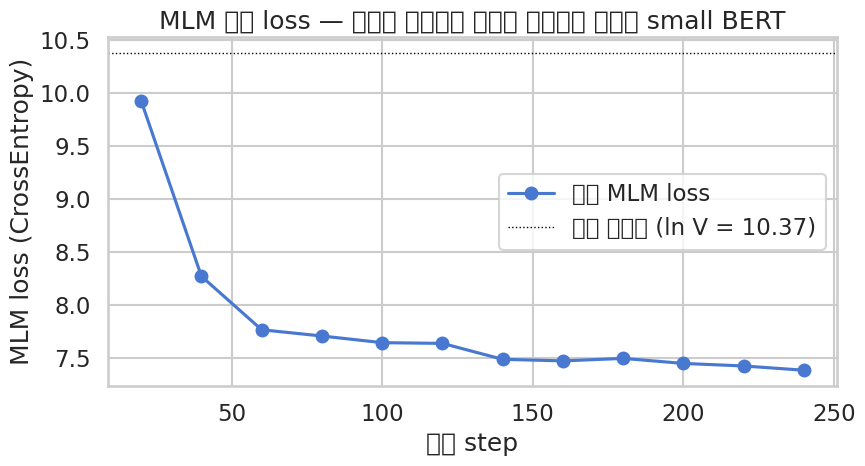
\includegraphics[width=0.82\linewidth]{assets/figures/ch22_mlm_training_loss.png}
\end{bookfigurelabel}

\textbf{그림 읽기} --- 그림~\ref{fig:ch22-mlm-training-loss}는 한국어 Wikipedia 문단으로 작은 BERT를 MLM 사전학습할 때의 train loss를 보여줍니다. 무작위 기준선 \(\log V\) 아래로 내려가는지가 핵심입니다. 절대값이 표준 \inlinecode{klue/bert-base} 수준에 도달하는지보다, 짧은 Colab 실습 안에서도 언어 모델 본체가 무작위 초기화 상태에서 벗어나는지를 확인하는 그림입니다.



\Needspace{11\baselineskip}
\begin{lstlisting}
eval_metrics = trainer.evaluate()
eval_loss = eval_metrics["eval_loss"]
eval_ppl = math.exp(eval_loss)
print(
    "=== eval (held-out Korean Wikipedia paragraphs) ==="
)
for k, v in eval_metrics.items():
    if isinstance(v, float):
        print(f"  {k:>22}: {v:.4f}")
print()
print(f"  MLM loss:               {eval_loss:.4f}")
print(f"  perplexity (exp loss):  {eval_ppl:.2f}")
print(
    f"  random baseline PPL:    "
    f"{tokenizer.vocab_size:,}  (uniform over vocab)"
)
\end{lstlisting}

\noindent\emph{앞 블록은 텍스트를 모델 입력 텐서로 바꾸는 단계입니다. 이어지는 블록에서는 앞에서 만든 중간 값을 다음 계산으로 넘기는 단계로 넘어갑니다.}

\Needspace{6\baselineskip}
\begin{lstlisting}[firstnumber=17]
print(
    f"  -> model narrowed vocab to approx. "
    f"{eval_ppl:.0f} candidates per masked position"
)
\end{lstlisting}

\noindent\textbf{출력.}
\begin{bookoutputbox}
Training Loss  Validation Loss  Epoch
-------------  ---------------  -----
7.424983       7.558918         2
=== eval (held-out Korean Wikipedia paragraphs) ===
               eval_loss: 7.5589

  MLM loss:               7.5589
  perplexity (exp loss):  1917.77
  random baseline PPL:    32,000  (uniform over vocab)
  -> model narrowed vocab to approx. 1918 candidates per masked position
\end{bookoutputbox}
\par\vspace{0.9em}

\section{사전학습 전후 비교}

학습 직전 (5-2 마지막 셀에서 측정해 둔 \inlinecode{pre\_eval\_loss} / \inlinecode{pre\_top5\_records}) 와 \emph{완전히 같은 문장·같은 평가 셋} 에 학습 후 모델을 적용해 두 결과를 나란히 봅니다. \emph{사전학습이 본체에 무엇을 새겼는가} 의 가장 직접적인 증거.



\Needspace{11\baselineskip}
\begin{lstlisting}
post_eval = trainer.evaluate()
post_eval_loss = post_eval["eval_loss"]
post_eval_ppl  = math.exp(post_eval_loss)

print("=" * 78)
print("AFTER pretraining  (2 epoch MLM)")
print("=" * 78)
print(
    f"  eval_loss       : {post_eval_loss:.4f}   (before: "
    f"{pre_eval_loss:.4f})"
)
print(
    f"  eval_perplexity : {post_eval_ppl:,.2f}        (before: "
    f"{pre_eval_ppl:,.0f})"
)
print(
\end{lstlisting}

\noindent\emph{앞 블록은 학습 설정을 만들고 학습 루프를 실행하는 단계입니다. 이어지는 블록에서는 모델 출력을 확률이나 예측값으로 바꾸는 단계로 넘어갑니다.}

\Needspace{11\baselineskip}
\begin{lstlisting}[firstnumber=17]
    f"  -> narrowed vocab to approx. "
    f"{post_eval_ppl:.0f} candidates per masked position"
)
print()

post_top5_records = []
for sent in test_sentences:
    results = predict_mask(sent, top_k=5)
    top5_tokens = [tok for tok, _ in results[0][1]] if results else []
    post_top5_records.append({"sentence": sent, "top5_after": top5_tokens})
    print(f"input: {sent}")
    print(f"  top-5 after pretraining: {top5_tokens}")
    print()
\end{lstlisting}

\noindent\textbf{출력.}
\begin{bookoutputbox}
Training Loss  Validation Loss  Epoch
-------------  ---------------  -----
7.424983       7.566011         2
==============================================================================
AFTER pretraining  (2 epoch MLM)
==============================================================================
  eval_loss       : 7.5660   (before: 10.4471)
  eval_perplexity : 1,931.42        (before: 34,446)
  -> narrowed vocab to approx. 1931 candidates per masked position

input: 대한민국의 수도는 [MASK]이다.
  top-5 after pretraining: ['.', ',', '##의', '##다', '##년']

input: 태양계에는 행성이 [MASK] 개 있다.
  top-5 after pretraining: ['.', '##의', ',', '##다', ')']
...
\end{bookoutputbox}
\par\vspace{0.9em}

\subsection{평가 손실과 perplexity}

두 측정치를 한 표·한 막대 그래프로.



\Needspace{10\baselineskip}
\begin{lstlisting}
metric_compare = pd.DataFrame({
    "metric":           ["eval_loss", "eval_perplexity"],
    "before (random)":  [pre_eval_loss,  pre_eval_ppl],
    "after (2 epoch)":  [post_eval_loss, post_eval_ppl],
    "random baseline":  [random_baseline_loss, float(tokenizer.vocab_size)],
})
print("Before vs After — eval metrics")
print(metric_compare.round(4).to_string(index=False))
\end{lstlisting}

\noindent\textbf{출력.}
\begin{bookoutputbox}
Before vs After — eval metrics
         metric  before (random)  after (2 epoch)  random baseline
      eval_loss          10.4471           7.5660          10.3735
eval_perplexity       34445.6443        1931.4213       32000.0000
\end{bookoutputbox}
\par\vspace{0.9em}
\Needspace{11\baselineskip}
\begin{lstlisting}
sns.set_theme(style="whitegrid", context="talk")
fig, axes = plt.subplots(1, 2, figsize=(12, 5))

loss_values = [pre_eval_loss, post_eval_loss]
loss_labels = ["before (random)", "after (2 epoch)"]
axes[0].bar(
    loss_labels,
    loss_values,
    color=["#999999", "#EE854A"],
)
axes[0].axhline(random_baseline_loss, color="black", lw=1.0, ls=":",
                label=f"random baseline ln V = {random_baseline_loss:.2f}")
axes[0].set_ylabel("eval_loss")
axes[0].set_title("MLM eval_loss")
axes[0].legend(loc="upper right", fontsize=10)

\end{lstlisting}

\noindent\emph{앞 블록은 숫자 결과를 그림으로 확인하는 단계입니다. 이어지는 블록에서는 텍스트를 모델 입력 텐서로 바꾸는 단계로 넘어갑니다.}

\Needspace{11\baselineskip}
\begin{lstlisting}[firstnumber=17]
ppl_values = [pre_eval_ppl, post_eval_ppl]
axes[1].bar(
    loss_labels,
    ppl_values,
    color=["#999999", "#EE854A"],
)
axes[1].set_yscale("log")
axes[1].axhline(tokenizer.vocab_size, color="black", lw=1.0, ls=":",
                label=f"random baseline V = {tokenizer.vocab_size:,}")
axes[1].set_ylabel("perplexity (log scale)")
axes[1].set_title("MLM perplexity")
axes[1].legend(loc="upper right", fontsize=10)

plt.tight_layout()
plt.show()
\end{lstlisting}

\noindent\textbf{출력.}
\begin{bookoutputbox}
<Figure size 1200x500 with 2 Axes>
\end{bookoutputbox}
\par\vspace{0.9em}
\begin{bookfigurelabel}[H]{한국어 MLM 평가 손실과 perplexity 변화}{fig:ch22-eval-loss-ppl}
\centering
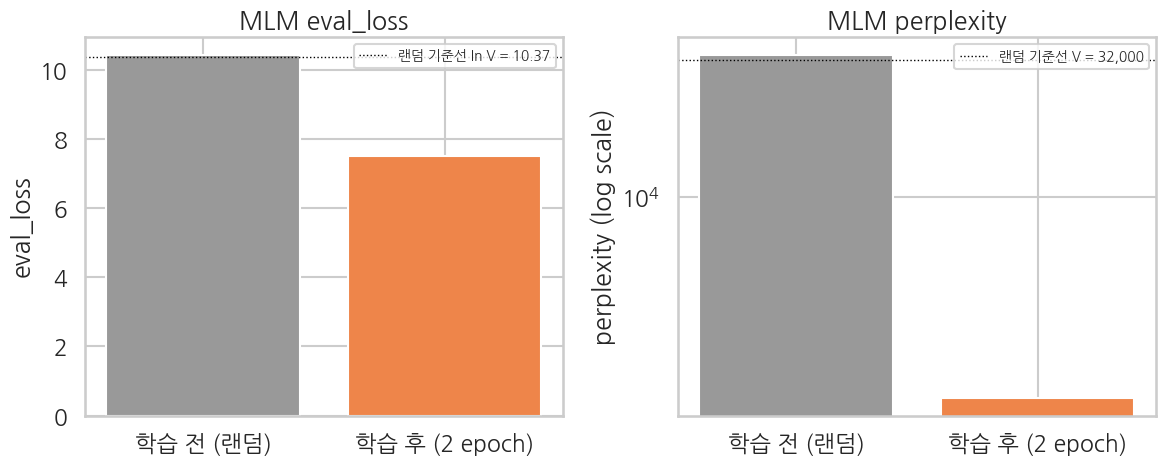
\includegraphics[width=0.82\linewidth]{assets/figures/ch22_eval_loss_ppl.png}
\end{bookfigurelabel}

\textbf{그림 읽기} --- 그림~\ref{fig:ch22-eval-loss-ppl}는 사전학습 전후의 평가 손실과 perplexity를 나란히 비교합니다. Perplexity는 로그 축으로 보아야 변화가 읽힙니다. 값이 낮아질수록 마스크 위치에서 가능한 후보 토큰 공간을 더 좁힌다는 뜻이며, 23장에서 이 본체를 분류 헤드와 연결할 준비가 됩니다.



\subsection{\texorpdfstring{표준 KLUE-BERT 기준점}{표준 KLUE-BERT 기준점}}

우리 작은 BERT (10M, 한국어 위키 5K paragraphs \(\times\) 2 epoch) 의 top-5 가 \emph{방향성은 맞지만 정답이 잘 안 보이는} 이유는 단순합니다 --- \textbf{학습 데이터·모델 크기·학습 시간 모두 부족}. \emph{그럼 학습이 충분히 잘 되면 어떤 결과가 나오나?} 의 답을 같은 한국어 문장에 표준 \inlinecode{klue/bert-base} (110M, 약 8.4B 토큰 대규모 한국어 코퍼스) 를 적용해 직접 봅니다.

같은 토크나이저 (\inlinecode{klue/bert-base}) 를 쓰고 있으므로 \emph{모델만 바꿔} 두 결과를 나란히.



\Needspace{11\baselineskip}
\begin{lstlisting}
from transformers import AutoModelForMaskedLM

ref_model = AutoModelForMaskedLM.from_pretrained("klue/bert-base")
ref_model.to(model.device)
ref_model.eval()

ref_param_count = sum(p.numel() for p in ref_model.parameters())
our_param_count = sum(p.numel() for p in model.parameters())
print(
    f"Our small BERT params: "
    f"{our_param_count/1e6:.1f}M"
)
print(
    f"Reference BERT params: {ref_param_count/1e6:.1f}M  ("
    f"{ref_param_count/our_param_count:.0f}x larger)"
)
\end{lstlisting}

\noindent\textbf{출력.}
\begin{bookoutputbox}
----------------------------+------------+--+-

Our small BERT params: 11.5M
Reference BERT params: 110.7M  (10x larger)
\end{bookoutputbox}
\par\vspace{0.9em}
\Needspace{11\baselineskip}
\begin{lstlisting}
def predict_mask_with(text, ref, top_k=5):
    '''임의의 MLM 모델로 [MASK] 자리 top-k 예측.'''
    ref.eval()
    inputs = tokenizer(text, return_tensors="pt").to(ref.device)
    with torch.no_grad():
        outputs = ref(**inputs)
    logits = outputs.logits[0]
    mask_positions = (inputs["input_ids"][0] == tokenizer.mask_token_id).nonzero(as_tuple=True)[0]
    if len(mask_positions) == 0:
        return None
    results = []
\end{lstlisting}

\noindent\emph{앞뒤 블록은 모두 텍스트를 모델 입력 텐서로 바꾸는 단계입니다. 길이를 나누어 같은 흐름을 단계별로 확인합니다.}

\Needspace{11\baselineskip}
\begin{lstlisting}[firstnumber=12]
    for pos in mask_positions:
        probs = torch.softmax(logits[pos], dim=-1)
        top_p, top_i = probs.topk(top_k)
        candidates = [(
            tokenizer.convert_ids_to_tokens(int(i)),
            float(p),
        )
                       for p, i in zip(top_p, top_i)]
        results.append((int(pos), candidates))
    return results

\end{lstlisting}

\noindent\emph{앞 블록은 텍스트를 모델 입력 텐서로 바꾸는 단계입니다. 이어지는 블록에서는 모델 출력을 확률이나 예측값으로 바꾸는 단계로 넘어갑니다.}

\Needspace{11\baselineskip}
\begin{lstlisting}[firstnumber=23]
ref_top5_records = []
for sent in test_sentences:
    results = predict_mask_with(sent, ref_model, top_k=5)
    top5_tokens = [tok for tok, _ in results[0][1]] if results else []
    ref_top5_records.append({"sentence": sent, "top5_ref": top5_tokens})

del ref_model
if torch.cuda.is_available():
    torch.cuda.empty_cache()
\end{lstlisting}



\subsection{{[}MASK{]} top-5 --- 3-way 비교 (before / ours / reference klue/bert-base)}

같은 한국어 문장 4개의 {[}MASK{]} 자리 top-5 후보를 \emph{사전학습 전 \(\to\) 우리 작은 BERT 학습 후 \(\to\) 표준 klue/bert-base} 셋으로 나란히.



\Needspace{10\baselineskip}
\begin{lstlisting}
rows = []
for pre, post, ref in zip(pre_top5_records, post_top5_records, ref_top5_records):
    rows.append({
        "sentence":          pre["sentence"],
        "top5_before":       ", ".join(pre["top5_before"]),
        "top5_ours":         ", ".join(post["top5_after"]),
        "top5_ref_bert":     ", ".join(ref["top5_ref"]),
    })

\end{lstlisting}

\noindent\emph{앞뒤 블록은 모두 앞에서 만든 중간 값을 다음 계산으로 넘기는 단계입니다. 길이를 나누어 같은 흐름을 단계별로 확인합니다.}

\Needspace{11\baselineskip}
\begin{lstlisting}[firstnumber=10]
top5_compare = pd.DataFrame(rows)
print(
    "Before (random) vs Ours (small BERT, ko wiki 5K) vs "
    "Reference (klue/bert-base, approx. 8.4B tokens)"
)
print("=" * 100)
for _, row in top5_compare.iterrows():
    print(f"input: {row['sentence']}")
    print(
        f"  before (random)            : "
        f"{row['top5_before']}"
    )
    print(
        f"  ours  (small, 5K para)     : "
        f"{row['top5_ours']}"
    )
\end{lstlisting}

\noindent\emph{앞뒤 블록은 모두 앞에서 만든 중간 값을 다음 계산으로 넘기는 단계입니다. 길이를 나누어 같은 흐름을 단계별로 확인합니다.}

\Needspace{7\baselineskip}
\begin{lstlisting}[firstnumber=26]
    print(
        f"  ref   (klue/bert-base)     : "
        f"{row['top5_ref_bert']}"
    )
    print()
\end{lstlisting}

\noindent\textbf{출력.}
\begin{bookoutputbox}
Before (random) vs Ours (small BERT, ko wiki 5K) vs Reference (klue/bert-ba...
===========================================================================...
input: 대한민국의 수도는 [MASK]이다.
  before (random)            : 서약, 정공, ##퐁, 회선, 슘
  ours  (small, 5K para)     : ., ,, ##의, ##다, ##년
  ref   (klue/bert-base)     : 서울, 광화문, 평양, 부산, 인천

input: 태양계에는 행성이 [MASK] 개 있다.
  before (random)            : 양봉, 선거전, ##yp, 나중, D
  ours  (small, 5K para)     : ., ##의, ,, ##다, )
  ref   (klue/bert-base)     : 여러, 몇, 두, 세, 다섯

input: 이 영화 정말 [MASK].
  before (random)            : 전유물, 대구, ##껄, 신기록, 학번
  ours  (small, 5K para)     : ., ,, ##의, ), ##다
  ref   (klue/bert-base)     : 좋아, [UNK], ., 좋아해, 좋아한다
...
\end{bookoutputbox}
\par\vspace{0.9em}
\textbf{해석 가이드 --- 사전학습이 만든 차이}

\begin{itemize}
\tightlist
\item
  \textbf{\inlinecode{eval\_loss}}: random baseline \(\ln V \approx 10.37\) 에서 약 5-7 부근까지 떨어졌으면 본체가 \emph{언어 구조 일부} 를 학습. \emph{완전한} 한국어 표상은 아니어도 \inlinecode{klue/bert-base} 가 학습한 것의 \emph{방향} 은 맞춤.
\item
  \textbf{\inlinecode{perplexity}}: 32,000 (vocab 전체) 에서 약 1,900 부근으로. \emph{마스크 자리마다 후보를 약 1,900개로 좁힌 상태} 라는 직관적 해석.
\item
  \textbf{top-5 토큰} (3-way 비교):

  \begin{itemize}
  \tightlist
  \item
    \emph{before (random)}: 자주 등장하는 \emph{조사·어미·특수문자} (\inlinecode{\#\#요}, \inlinecode{\#\#어}, \inlinecode{.}, \inlinecode{는}, \inlinecode{이}) --- random init 이지만 logits 가 미세하게 흔들려 \emph{통계적 빈도} 높은 토큰만 뽑힘.
  \item
    \emph{ours (small BERT, 위키 5K paragraphs \(\times\) 2 epoch)}: 한국어 어미·내용어 일부가 섞이기 시작 --- 위키 도메인은 \emph{방향성이 보이지만} 정답 (\inlinecode{서울}, \inlinecode{8} 등) 이 top-5 안에 \emph{안정적으로} 들어오지는 못함. \textbf{데이터·모델 크기 부족의 한계}.
  \item
    \emph{ref (klue/bert-base, 약 8.4B 토큰)}: 위키 도메인은 \emph{정답이 top-1} --- \inlinecode{서울}, \inlinecode{여덟} 같은 자연스러운 답. NSMC 도메인 (다른 도메인) 도 \emph{감성 형용사·부사} (\inlinecode{재미있}, \inlinecode{정말}, \inlinecode{너무}) 가 자연스럽게 top-5 에 들어옴. \textbf{이게 사전학습이 충분히 잘 됐을 때의 모습}.
  \end{itemize}
\end{itemize}

\begin{quote}
\textbf{세 모델의 격차가 정확히 \emph{데이터 규모 + 모델 크기 + 학습 시간} 의 격차} --- 우리 작은 BERT (10M, 위키 5K paragraphs, 2 epoch) \(\to\) reference (110M, 약 8.4B tokens) 사이에 \emph{데이터 수천 배, 파라미터 11배}. 그 격차가 top-5 의 \emph{질적 차이} 로 정확히 드러납니다.
\end{quote}

이 장의 작은 BERT 는 \emph{한국어 위키 paragraphs 5K \(\times\) 2 epoch} 로 학습한 \emph{일반 도메인 mini BERT}. 위키 도메인은 직접 본 분포라 향상이 빠르지만, NSMC 영화 리뷰는 \emph{다른 도메인} 이라 fine-tune 단계에서 적응이 필요합니다 --- 이게 \emph{진짜 사전학습 \(\to\) fine-tune 패러다임} 의 핵심. \ref{ch:23}장에서 NSMC 이진 분류로 fine-tune 할 때 진짜 비교 --- \emph{우리가 직접 만든 작은 한국어 BERT (일반 도메인 5K, 약 10M)} vs \emph{\ref{ch:15}장의 \inlinecode{klue/bert-base} (대규모 일반 코퍼스, 약 110M)}.



\section{모델 저장 --- \ref{ch:23}장에서 재사용}

\inlinecode{model.save\_pretrained()} 와 \inlinecode{tokenizer.save\_pretrained()} 를 \emph{같은 폴더} 에 저장. \ref{ch:23}장에서는 \inlinecode{AutoModelForSequenceClassification.from\_pretrained("./ch22\_small\_bert\_mlm\_ko",\ num\_labels=2)} 한 줄로 \emph{이 BERT body} 를 가져와 분류 헤드를 새로 얹습니다.



\Needspace{11\baselineskip}
\begin{lstlisting}
SAVE_DIR = "./ch22_small_bert_mlm_ko"
model.save_pretrained(SAVE_DIR)
tokenizer.save_pretrained(SAVE_DIR)

import os
print(f"Saved to: {SAVE_DIR}")
print(f"Files:")
for f in sorted(os.listdir(SAVE_DIR)):
    size = os.path.getsize(os.path.join(SAVE_DIR, f))
    if size > 1024 * 1024:
        size_str = f"{size / 1024 / 1024:.1f} MB"
    else:
        size_str = f"{size / 1024:.1f} KB"
    print(f"  {f:>30s}  {size_str}")
\end{lstlisting}

\noindent\textbf{출력.}
\begin{bookoutputbox}
Saved to: ./ch22_small_bert_mlm_ko
Files:
                     config.json  0.7 KB
               model.safetensors  43.8 MB
                  tokenizer.json  734.4 KB
           tokenizer_config.json  0.4 KB
\end{bookoutputbox}
\par\vspace{0.9em}
\textbf{저장된 파일 구조} --- \ref{ch:20}장과 동일한 HF 표준 레이아웃:

\begin{booktable}{22장 모델 저장과 다음 장 재사용}{tab:ch22-06}
\begin{adjustbox}{max width=\textwidth}
\begin{tabular}{@{}ll@{}}
\toprule
파일 & 역할 \\
\midrule

\inlinecode{config.json} & \inlinecode{BertConfig} 직렬화 (hidden, layer, head, vocab 등) \\
\inlinecode{model.safetensors} (또는 \inlinecode{pytorch\_model.bin}) & 모델 weight \\
\inlinecode{tokenizer.json} / \inlinecode{vocab.txt} & 한국어 토크나이저 (\ref{ch:23}장 fine-tune 에서 동일 사용) \\
\inlinecode{special\_tokens\_map.json}, \inlinecode{tokenizer\_config.json} & 특수 토큰 메타 \\
\bottomrule
\end{tabular}
\end{adjustbox}
\end{booktable}

\begin{quote}
\ref{ch:23}장에서 \inlinecode{AutoModelForSequenceClassification.from\_pretrained("./ch22\_small\_bert\_mlm\_ko",\ num\_labels=2)} 호출 시, \inlinecode{BertForMaskedLM} 의 \emph{MLM head 는 버려지고} encoder body 만 가져옴. 그 위에 새 \inlinecode{Linear(256,\ 2)} 분류 헤드를 random init 으로 부착. \ref{ch:15}장의 \inlinecode{klue/bert-base} fine-tune 과 \emph{같은 구조} --- 본체 출발점 (사전학습 규모) 만 다름.
\end{quote}



\section{변형: 데이터와 학습량}

작은 BERT 의 성능은 \emph{학습량} 에 민감합니다. T4 30분 룰 안에서 가능한 변형:

\begin{booktable}{22장 변형: 데이터와 학습량 표}{tab:ch22-07}
\begin{adjustbox}{max width=\textwidth}
\begin{tabular}{@{}llll@{}}
\toprule
변형 축 & 이 장 (기본) & 변형 예 & 예상 효과 \\
\midrule

\inlinecode{N\_TRAIN\_TEXT} & 5,000 & 30,000 & 한 epoch 시간 약 6배, loss 하락폭 큼. 30분 안엔 1 epoch 만 가능 \\
\inlinecode{num\_train\_epochs} & 2 & 3 & eval loss 약간 하락, perplexity 약 2-3 정도 감소 \\
\inlinecode{BLOCK\_SIZE} & 128 & 64 & 블록 수 약 2배 증가, 한 블록 짧아져 \emph{문맥} 줄음 \\
\inlinecode{mlm\_probability} & 0.15 & 0.20-0.25 & 한국어는 형태소 풍부해 \emph{가릴 자리} 가 많음. 학습 신호 약간 늘지만 trade-off 있음 (FAQ Q2 참고) \\
데이터 출처 & 한국어 Wikipedia (5K paragraphs) & 더 많은 위키 + 모두의 말뭉치 + 뉴스 & klue/bert-base 의 약 8.4B 토큰에 더 가까이 --- 단, 토큰 수 늘리면 학습 시간 비례 증가 \\
\bottomrule
\end{tabular}
\end{adjustbox}
\end{booktable}

\begin{quote}
\textbf{T4 30분 룰 안에서 가능한 가장 큰 개선} --- \inlinecode{N\_TRAIN\_TEXT\ =\ 20000}, 1 epoch 정도가 한계. \ref{ch:23}장에서 \emph{얼마나 도움 됐는지} 가 진짜 검증.
\end{quote}



\section{이 장에 등장한 라이브러리·함수 (\ref{ch:20}장과의 차이만)}

\begin{booktable}{22장 새로 등장한 라이브러리}{tab:ch22-08}
\begin{adjustbox}{max width=\textwidth}
\begin{tabular}{@{}lll@{}}
\toprule
이름 & 한 줄 설명 & \ref{ch:20}장과 차이 \\
\midrule

\inlinecode{AutoTokenizer.from\_pretrained("klue/bert-base")} & 한국어 WordPiece (vocab 약 32,000) & 영어 \(\to\) 한국어 \\
\inlinecode{load\_dataset("wikimedia/wikipedia",\ "20231101.ko")} & 한국어 Wikipedia HF 정제본 로드 & \inlinecode{load\_dataset("Salesforce/wikitext",\ ...)} (\ref{ch:20}장) --- 같은 패턴, 언어만 변경 \\
\texttt{Dataset.from\_pandas(df{[}{[}"document"{]}{]}).rename\_column(...)} & pandas \(\to\) HF Dataset 변환 & \ref{ch:15}장과 같은 패턴 \\
\inlinecode{transformers.BertConfig} (동일) & 작은 BERT hyperparam & (\ref{ch:20}장 동일) \\
\inlinecode{transformers.BertForMaskedLM(config)} (동일) & random init MLM 모델 & (\ref{ch:20}장 동일) \\
\inlinecode{DataCollatorForLanguageModeling(mlm\_probability=0.15)} (동일) & 매 batch 동적 80/10/10 masking & (\ref{ch:20}장 동일) \\
\inlinecode{group\_texts} 패턴 (동일) & 가변 길이 \(\to\) 고정 블록 스트림 & (\ref{ch:20}장 동일) \\
\inlinecode{model.save\_pretrained()} / \inlinecode{tokenizer.save\_pretrained()} (동일) & HF 표준 체크포인트 & (\ref{ch:20}장 동일) \\
\bottomrule
\end{tabular}
\end{adjustbox}
\end{booktable}



\section{체크포인트 질문}

\begin{enumerate}
\def\labelenumi{\arabic{enumi}.}
\tightlist
\item
  \ref{ch:19}장 §5-4 에서 \emph{영어 토크나이저로 한국어를 토큰화하면 UNK 가 폭증} 한다는 걸 봤습니다. 이 장의 토크나이저 비교 표 (셀 2 하단) 가 그 결론과 정확히 일치하나요? \inlinecode{bert-base-uncased} 가 한국어 문장을 \emph{자모 단위} 로 분해한 결과를 어떻게 해석해야 할까요?
\item
  MLM random baseline 이 \ref{ch:20}장 (vocab 30,522) 의 약 10.33 에서 \ref{ch:22}장 (vocab 32,000) 의 약 10.37 로 \emph{미세하게} 바뀝니다. 이 0.04 차이가 학습 동역학에 의미 있는 영향을 주나요? (힌트: 학습 곡선의 절대값 vs 상대 변화)
\item
  한국어 위키 paragraph 는 \emph{제한 50-2000자 필터} 로 평균 길이가 일정합니다. NSMC 한 줄 리뷰보다 길고 Yelp 보다는 짧음. 같은 5K 샘플이라도 \emph{총 토큰 양} 이 \ref{ch:20}장 (Yelp) 와 어떻게 다른지, 같은 epoch 수에서 \emph{생성 블록 수} 가 어떻게 달라지는지 확인해 보세요.
\item
  \inlinecode{DataCollatorForLanguageModeling} 이 토큰 id 만 보고 동작한다는 게 이 장의 결론 중 하나입니다. 그렇다면 \emph{한국어 모델 학습 시 mlm\_probability 를 0.15 가 아닌 다른 값으로 바꿔야 할 이유} 가 있을까요?
\end{enumerate}



\section{FAQ}

\begin{faqBox}{Q1. (실무) \inlinecode{bert-base-uncased} 토크나이저를 그대로 쓰면 안 되나요? \ref{ch:20}장의 코드를 \emph{언어만 데이터로} 바꾸는 게 더 단순한데.}

쓰면 \emph{거의 학습 안 됨} 입니다. 이 장 셀 2 하단의 비교 표가 그 답:

\Needspace{8\baselineskip}
\begin{lstlisting}
tokenizer_en = AutoTokenizer.from_pretrained("bert-base-uncased")
sent = "이 영화 정말 재미있어요!"
toks = tokenizer_en.tokenize(sent)
# ['jamo_1', '##jamo_2', 'jamo_3', '##jamo_4',
#  '##jamo_5', '##jamo_6', '##jamo_7', '[UNK]',
# '!']
\end{lstlisting}

한국어 문장이 \emph{자모 단위} 로 분해되거나 \texttt{{[}UNK{]}} 가 섞입니다. 임베딩 테이블이 \emph{vocab 30,522 영어 단어 위주} 라 자모·UNK 자리의 임베딩이 \emph{의미 없는 random vector}. 그 위에서 MLM 학습을 해도 \emph{언어 정보를 압축할 자리} 가 없습니다. \ref{ch:19}장 §5-4 의 결론을 그대로 재확인 --- \emph{토크나이저는 모델의 언어를 물리적으로 결정} 합니다.

\end{faqBox}

\begin{faqBox}{Q2. (이론) 한국어는 형태소가 풍부한데 \inlinecode{mlm\_probability} 를 0.20-0.25 로 올리면 학습이 더 잘 되나요?}

\textbf{일부 연구는 그런 시도를 했고 결과는 trade-off} 입니다. 한국어는 한 어절 안에 \emph{어간 + 어미 + 조사} 가 결합되어 형태소 정보가 풍부 \(\to\) 가릴 자리가 많아 \emph{학습 신호 양} 은 늘 수 있습니다. 그러나:

\Needspace{7\baselineskip}
\begin{lstlisting}
data_collator = DataCollatorForLanguageModeling(
    tokenizer=tokenizer,
    mlm=True,
    mlm_probability=0.25,
)
\end{lstlisting}

\begin{itemize}
\tightlist
\item
  \textbf{장점}: 한 batch 당 학습되는 토큰 수가 약 1.7배 증가 \(\to\) loss 가 같은 step 수에서 더 빨리 떨어질 수 있음
\item
  \textbf{단점}: 가려진 비율이 높으면 \emph{주변 문맥} 자체가 줄어들어 \emph{추측 가능성} 이 떨어짐. 모델이 \emph{의미 없는 random guess} 만 학습할 위험
\end{itemize}

BERT 논문의 15\% 는 \emph{모든 언어에서 합리적 sweet spot} 으로 정착했고, 한국어 BERT (\inlinecode{klue/bert-base}) 도 15\% 로 사전학습. \emph{0.20-0.25 시도는 가능} 하지만 \emph{명확한 개선 보장은 없음}. 작은 모델 + 작은 데이터일수록 \emph{기본 셋업 안정} 이 더 가치 있습니다.

\end{faqBox}

\begin{faqBox}{Q3. (이론) \inlinecode{klue/bert-base} 가 이미 학습된 모델인데 왜 같은 구조의 mini 버전을 처음부터 다시 학습하나요?}

\textbf{교육 목적} 입니다. 사전학습이 본체에 무엇을 새기는지 \emph{직접 경험} 하기 위해.

\Needspace{11\baselineskip}
\begin{lstlisting}
model = AutoModelForSequenceClassification.from_pretrained(
    "klue/bert-base",
    num_labels=2,
)

config = BertConfig(
    hidden_size=256,
    num_hidden_layers=4,
    ...,
)
model = BertForMaskedLM(config)
\end{lstlisting}

실무에서는 \emph{클루 본체 그대로 가져다 쓰는 게} 답입니다 --- 데이터·연산이 \emph{5000배 이상} 격차. 본 장의 목적은 \emph{그 격차의 의미} 를 \ref{ch:23}장에서 정량 비교하기 위함이고, \emph{작은 모델 + 작은 데이터로도 사전학습 동역학을 재현} 할 수 있음을 확인하는 것. \ref{ch:20}장 (영어) 의 한국어 대칭본.

\end{faqBox}

\begin{faqBox}{Q4. (실무) 한국어 텍스트에 영어가 섞여 있으면 \inlinecode{klue/bert-base} 토크나이저가 잘 처리하나요?}

대체로 잘 처리합니다 --- \inlinecode{klue/bert-base} 의 vocab 약 32,000 안에 영어 단어·서브워드도 일부 포함되어 있어 \emph{자주 등장하는 영어} 는 자연스럽게 토큰화됩니다. 다만:

\Needspace{5\baselineskip}
\begin{lstlisting}
mixed = "이 movie 정말 amazing 했어요!"
print(tokenizer.tokenize(mixed))
\end{lstlisting}

\begin{itemize}
\tightlist
\item
  \emph{자주 쓰는 영단어} (\inlinecode{movie}, \inlinecode{OK} 등): 1 토큰 또는 짧은 WordPiece 로 처리
\item
  \emph{드문 영단어} 나 \emph{고유명사}: 자모 단위 분해 또는 \texttt{{[}UNK{]}} 위험
\item
  \emph{한자, 일본어, 특수문자}: vocab 안에 일부만 있어 \emph{부분 UNK} 가능
\end{itemize}

한국어 위키 본문은 \emph{순한국어 + 인명·지명·과학 용어 등 영문 표기} 가 자주 섞입니다. \inlinecode{klue/bert-base} vocab 에 자주 쓰는 영단어 일부가 있어 큰 문제는 없습니다. 다국어 환경이라면 \emph{multilingual BERT} (\inlinecode{bert-base-multilingual-cased}) 또는 \emph{byte-level BPE} (XLM-R) 같은 \emph{공통 vocab} 모델을 고려.

\end{faqBox}

\begin{faqBox}{Q5. (이론) 셀 5-1 에서 본 \inlinecode{label\_id\ =\ -100} 이 정확히 어떻게 \emph{loss 무시} 로 이어지나요?}

PyTorch \inlinecode{CrossEntropyLoss} 의 기본 \inlinecode{ignore\_index=-100} 동작:

\Needspace{8\baselineskip}
\begin{lstlisting}
import torch
loss_fn = torch.nn.CrossEntropyLoss()
# ignore_index=-100 (default)
logits = torch.randn(10, 32000)         # (seq_len, vocab)
labels = torch.tensor([5, 9, -100, -100, 12, -100, -100, 7, -100, -100])
loss = loss_fn(logits, labels)
\end{lstlisting}

\inlinecode{DataCollatorForLanguageModeling} 이 가려지지 않은 자리에 \inlinecode{-100} 을 채우는 게 \emph{전 자리에서 CE 계산 후 마스킹} 보다 효율적입니다. 같은 트릭이:

\begin{itemize}
\tightlist
\item
  \textbf{GPT 사전학습} (24-26장): \inlinecode{labels\ =\ input\_ids.clone()} \(\to\) 사실상 \emph{모든 자리} 학습 (pad 만 -100)
\item
  \textbf{SFT / Instruction Tuning} (27장): \texttt{labels{[}prompt\_mask{]}\ =\ -100} \(\to\) \emph{답변 부분만} 학습
\end{itemize}

세 곳 모두 같은 \inlinecode{-100} 트릭, 적용 자리만 다릅니다. \ref{ch:21}장 §3 의 \emph{labels = -100 thread} 마크다운에 풀버전 설명.

\end{faqBox}

\begin{faqBox}{Q6. (실무) MLM eval loss 가 4-6 부근에서 \emph{더 떨어지지 않으면} 어떻게 진단하나요?}

작은 BERT scratch + 5K 문장의 \emph{자연스러운 수렴 영역} 입니다. 추가로 떨어뜨리려면:

\Needspace{7\baselineskip}
\begin{lstlisting}
N_TRAIN_TEXT = 30000

NUM_EPOCHS = 3

HIDDEN_SIZE = 384
\end{lstlisting}

데이터·epoch·모델 크기를 \emph{함께} 늘려야 효과가 큽니다. 단, T4 30분 룰 한계 --- \emph{원리 확인용 toy 셋업} 임을 잊지 말 것. 실제 한국어 사전학습은 \inlinecode{klue/bert-base} (한국어 위키 + 뉴스 + 댓글, 약 수억 토큰, GPU·TPU 수일) 가 한 결과물.

\end{faqBox}

\begin{faqBox}{Q7. (이론) \ref{ch:20}장 (영어) 와 \ref{ch:22}장 (한국어) 의 학습 곡선을 \emph{비교} 하려면 어떻게 해야 하나요?}

같은 hyperparam·같은 BLOCK\_SIZE·같은 epoch 으로 학습된 두 모델의 \emph{상대} 비교가 의미 있습니다.

\Needspace{11\baselineskip}
\begin{lstlisting}
metrics = {
    "language":           ["EN (20장)",    "KO (22장)"],
    "vocab_size":         [30522,           32000],
    "random_baseline":    [10.33,           10.37],
    "epoch1_eval_loss":   ["measure",       "measure"],
    "epoch2_eval_loss":   ["measure",       "measure"],
    "epoch2_perplexity":  ["measure",       "measure"],
    "train_tokens":       ["approx 700K",   "approx 500K"],
}
\end{lstlisting}

한국어 위키 paragraphs 는 평균 길이가 Yelp 리뷰보다 짧지만 NSMC 보다는 깁니다. 같은 5K 샘플이라도 \emph{토큰 총량} 이 Yelp 와 살짝 다릅니다. 같은 step 수에 \emph{실제 본 토큰 수} 가 다르고, eval loss 도 영향을 받습니다. \emph{언어 자체의 어려움 차이} 가 아니라 \emph{데이터 크기 차이} 가 더 큰 영향. 공정한 언어 비교는 \emph{토큰 총량 매칭} 이 필요.
\end{faqBox}



\begin{previewBox}{미리보기: 다음 장}

\textbf{\ref{ch:23}장. 작은 BERT 분류 --- 한국어 NSMC 이진 (일반 도메인 사전학습 \(\to\) 다른 도메인 fine-tune)}

\begin{itemize}
\tightlist
\item
  이 장의 \inlinecode{./ch22\_small\_bert\_mlm\_ko} 체크포인트를 \inlinecode{AutoModelForSequenceClassification.from\_pretrained(...,\ num\_labels=2)} 로 로드 \(\to\) MLM head 떼고 분류 헤드 부착
\item
  NSMC 이진 분류 fine-tune (\ref{ch:15}장과 같은 데이터·셋업) --- \emph{완전히 다른 도메인 transfer}
\item
  \textbf{핵심 비교}: 이번 작은 사전학습 BERT (약 10M params, 위키 5K paragraphs MLM) vs \ref{ch:15}장의 \inlinecode{klue/bert-base} (약 110M params, 대규모 일반 한국어 사전학습) --- 2-way
\item
  영어 \ref{ch:20}장 \(\to\) \ref{ch:21}장 흐름의 \emph{한국어 대칭본} --- 같은 격차 패턴이 한국어 환경에서도 나오는지 검증
\item
  추가로 \emph{random init baseline} 비교 + \emph{위키 \(\to\) NSMC 의 negative transfer 분석} 은 \ref{ch:23}장 부록 \href{../23_ko_bert_classify/appendix_random_baseline.ipynb}{\inlinecode{appendix\_random\_baseline.ipynb}}
\end{itemize}

\begin{quote}
\textbf{변하는 축}: Phase 3 안에서 \emph{task} 가 사전학습 (MLM) \(\to\) 분류 (fine-tune) 로 전환. \emph{파인튜닝} 의 의미는 \textbf{BERT 단계 = task 별 head 부착}. 본체는 그대로, downstream task 마다 새로 random init 된 작은 head 가 붙어 적응. \ref{ch:23}장에서 본격적으로 다시 짚어 봅니다.
\end{quote}
\end{previewBox}
